%%
%% 研究報告用スイッチ
%% [techrep]
%%
%% 欧文表記無しのスイッチ(etitle,eabstractは任意)
%% [noauthor]
%%

%\documentclass[submit,techrep]{ipsj}
\documentclass[submit,techrep,noauthor]{ipsj}



\usepackage[dvips]{graphicx}
\usepackage{latexsym}
\usepackage{indentfirst}
\usepackage{amsmath}
\usepackage{bm}
\usepackage{float}
\usepackage{multirow}
\usepackage{mathtools}
\usepackage{cite}
\usepackage{subfigure}

% ************************* ソースコード貼り付け用 *************************
\usepackage{listings}
\usepackage{ifthen}

\makeatletter
\let\MYcaption\@makecaption
\makeatother

\usepackage{caption}

\makeatletter
\let\@makecaption\MYcaption
\makeatother

% ソースコードで図番号を切り替えるためにカウンタを定義
\newcounter{sourcecodefigure}
\newcounter{normalfigure}

% カウンタの切り替えマクロ
\newcommand{\switchtosourcecode}{%
    \setcounter{normalfigure}{\value{figure}}
    \setcounter{figure}{\value{sourcecodefigure}}
}

\newcommand{\switchtonormal}{%
    \setcounter{sourcecodefigure}{\value{figure}}
    \setcounter{figure}{\value{normalfigure}}
}

\newcommand\sourcecodeposition{h}
\newenvironment{sourcecode}[1][h]{%
    \begin{figure}[#1]
    \renewcommand\sourcecodeposition{#1}
    \centering
    \captionsetup{name=ソースコード}
    \switchtosourcecode
    \ifthenelse{\equal{\sourcecodeposition}{t}}%
        {\vspace{-1.3zh}} % for 't'
        {\ifthenelse{\equal{\sourcecodeposition}{b}}%
            {\vspace{-2zh}} % for 'b'
            {\vspace{-2zh}} % for 'h' or default
    }
}{%
    \ifthenelse{\equal{\sourcecodeposition}{t}}%
        {\vspace{-1.3zh}} % for 't'
        {\ifthenelse{\equal{\sourcecodeposition}{b}}%
            {\vspace{-1zh}} % for 'b'
            {\vspace{-3zh}} % for 'h' or default
    }
    \switchtonormal
    \end{figure}
}

\lstset{
  basicstyle={\ttfamily},               % 基本:等幅フォント
  identifierstyle={\small},             % 識別子
  commentstyle={\smallitshape},         % コメント:斜体
  keywordstyle={\small\bfseries},       % キーワード:太字
  stringstyle={\small\ttfamily},        % 文字列
  frame={tb},                           % 上部と下部に線を表示
  breaklines=true,                      % 行が長い場合に折り返す
  columns=[l]{fullflexible},            % 列幅を自動調整する(見た目が良くなる)
  numbers=left,                         % 行番号を左側に表示
  xrightmargin=0zw,                     % 右マージンのサイズ.
  xleftmargin=1.6zw,                    % 左マージンのサイズ.行番号が2桁でも行左端からはみ出ない値.
  numberstyle={\scriptsize},            % 行番号のスタイル.スクリプトサイズのフォントを使用
  stepnumber=1,                         % 何行ごとに行番号を表示するか
  numbersep=1zw,                        % 行番号とソースコードの間の距離
  lineskip=-1.4ex,                      % ソースコードの行間(結構詰め気味)
}
% ************************* ソースコード貼り付け用 *************************

\def\Underline{\setbox0\hbox\bgroup\let\\\endUnderline}
\def\endUnderline{\vphantom{y}\egroup\smash{\underline{\box0}}\\}
\def\|{\verb|}
%

\begin{document}

\title{組合せ最適化問題のための疑似量子\\アニーリングマシンの制約機能に関する検討}

\author{伴内 光太郎}{Kotaro Bannai}{IPSJ}[東北大学グリーンクロステック研究センター\\Green\,Cross-Tech\,Research\,Center{,}\,Tohoku University]
\author{小松 一彦}{Komatsu Kazuhiko}{IPSJ}
\author{中曽根 才将}{Nakasone Takamasa}{IPSJ}[日本電気株式会社\\NEC\,Corporation]
\author{百瀬 真太郎}{Momose Shintaro}{IPSJ}
\author{小林 広明}{Kobayashi Hirokaki}{IPSJ}[東北大学サイバーサイエンスセンター\\Cyberscience\,Center{,}\,Tohoku University]

\begin{abstract}
組合せ最適化問題を高速に解く一つの手段として, デジタル回路上に実装された疑似量子アニーリングマシンが注目されている. 近年開発された疑似量子アニーリングマシンでは, 制約条件を含む最適化問題に対して, 制約条件を一般的な入力形式であるQUBO (Quadratic Unconstrained Binary Optimization) とは独立に指定することにより
, 探索時に制約を考慮しつつ最適解を効率的かつ高速に求解できる機能を有している. 一方, この制約機能が疑似量子アニーリングマシンにおける全体の性能にどのように影響を与えるかについては詳細な検証がなされていない. 本稿では, 組合せ最適化問題において頻出するワンホット制約, 不等式制約, 禁止ペア制約に対して, 疑似量子アニーリングマシンが持つ制約機能の重要性を明らかにし, 各制約に応じて適切な機能を利用することが重要であることを明らかにした.
\end{abstract}

\maketitle

%1
\section{はじめに}
組合せ最適化問題は, 制約条件のもと多数の組み合わせの中から目的関数を最小化する変数の組み合わせを求める問題であり, 生産順序最適化\cite{jobshop},配送ルート最適化\cite{isc-onoda},金融ポートフォリオ最適化\cite{portfolio}など現実の様々な社会課題に応用できるとして期待されている. 組合せ最適化問題の多くはNP困難であり, 問題規模が大きくなると現実的な時間で最適解を求めることは難しい. 近年, 組合せ最適化問題を高速に解く一つの手段として, デジタル回路上に実装された疑似量子アニーリングマシンが注目されている. 疑似量子アニーリングマシンを用いた最適化では, 問題をQUBO (Quadratic Unconstrained Binary Optimization) と呼ばれる物理モデルにより表現し, QUBOを疑似量子アニーリングマシンに投入することで最適な変数の解を得る.

一方, QUBOによる問題表現では, 制約条件をペナルティ関数としてQUBOによるエネルギー関数の一部に埋め込む必要がある. ペナルティ関数の導入は通常, 最適解の探索精度に影響に与えることから, 標準的なアニーリングマシンでは, 制約条件を含む問題において高精度な解を得ることは一般的に難しいとされる\cite{ozeki, onoda2}.

この問題に対して, 近年開発された疑似量子アニーリングマシンでは, 制約条件の情報をQUBOとは独立に指定することにより, 探索時に制約条件を考慮しつつ最適解をより効率的かつ高速に求解できる機能が搭載されている\cite{takano, da3}. このような機能は, 現存のD-Wave社による量子アニーリングマシンでは提供されておらず, デジタル回路上に実装された疑似量子アニーリングマシンに特有の機能である. 

本稿では, 組合せ最適化問題における制約部分に着目し, 組合わせ最適化問題において頻出するワンホット制約, 不等式制約, 禁止ペア制約に対する疑似量子アニーリングマシンの制約機能の有効性を明らかにする.

本稿の構成は,以下の通りである.2章では, QUBOの概要, 及び異なる制約条件を含む組合せ最適化問題の概要について述べる. 3章では,疑似量子アニーリングマシンの概要, 各制約条件に対応する疑似量子アニーリングマシンの制約機能について述べる. 4章では,評価環境及び性能評価結果を示す.5章では本検討のまとめを述べる.

%2
\section{組合せ最適化問題}

%2.1
\subsection{QUBO}
\textcolor{blue}{QUBOは0または1を取るバイナリ変数の二次多項式で系全体のエネルギーを記述するモデルであり, バイナリ変数を$x_{i}\in\{0, 1\}$と定義した場合, 以下の通り記述される.
\begin{equation}
H_{\rm{QUBO}}(\bm{x}) = \sum_{(i,j)} Q_{i,j}x_{i}x_{j}
\label{H_qubo}
\end{equation}
ここで$Q_{i,j}$は相互作用係数である. 組合せ最適化問題において, バイナリ変数$x_{i}$は, 相反する二つの事象を表す決定変数に対応している. 係数$Q_{i,j}$は, 組合せ最適化問題を特徴付ける量であり, 後述の擬似量子アニーリングマシンは, $Q_{i,j}$を入力として全体のエネルギー関数が最小となる決定変数の解を探索する. }

\textcolor{blue}{QUBOでは, 組合せ最適化問題における制約条件をペナルティ関数として目的関数と共に係数$Q_{i,j}$に含めて定式化を行う. 制約条件を含む組合せ最適化問題における一般的なエネルギー関数は, 目的関数によるエネルギー関数$H_{\rm{obj}}(\bm{x})$, 及び制約条件に対するペナルティ関数$H_{\rm{pen}}(\bm{x})$を用いて, 以下の通り記述される.
\begin{equation}
H_{\rm{QUBO}}(\bm{x}) = H_{\rm{obj}}(\bm{x}) + \lambda H_{\rm{pen}}(\bm{x})
\label{H_qubo}
\end{equation}
ここで, $\lambda$はペナルティ関数に乗じられる重みを表す. $H_{\rm{pen}}(\bm{x})$は通常, 制約条件を違反する状態に対してエネルギーを増加させる関数により記述される. このため, 制約の重み$\lambda$には, 制約違反を防ぐために十分大きい値を指定する必要がある. 一方, ペナルティ関数の導入は通常, エネルギー関数のランドスケープを複雑化する方向に作用するため, QUBOにおける制約条件の取り扱いは一般的に難しく, 高精度な解が得られにくいとされる\cite{kumagai, komatsu, kumagai2}. } 

\textcolor{blue}{一方, 制約条件は, 実問題における前提や要件を指定するためによく用いられており, その中でも特にワンホット制約, 不等式制約, 禁止ペア制約は多くの最適化問題において頻出する重要な制約条件である. 次節以降では, 導入として制約条件を含まない最適化問題のQUBO定式化について述べた後, 各制約条件を含む代表的な最適化問題のQUBO定式化をそれぞれ紹介する.}

%2.2
\subsection{制約なし最適化問題}

%2.2.1
制約なし最適化問題は, 決定変数を選択する範囲にいかなる制約条件を含まず, 目的関数の最大化及び最小化のみを目的とした最適化問題である. 制約なし最適化問題の一つとして, 最大カット(Maxcut)問題 が知られている. Maxcutは, 頂点集合$V$と辺集合$E$を持つ無向グラフ$G(V,E)$が与えられたとき, $V$を2つの集合に分割することで2つの集合間の辺の数(各辺に重みが与えられている場合は重みの総和)ができるだけ大きくなるようにする問題である\cite{maxcut}. グラフに関する典型的な最適化問題であり, 画像処理や通信網・交通網等のネットワーク計画等に応用される.

MaxcutのQUBO定式化は, 頂点$i$が集合に含まれる場合に1,もう一方の集合に含まれる場合に0を満たすバイナリ変数$x_{i}$を用いることで,以下の通り記述される. 
\textcolor{blue}{
\begin{align}
H_{\rm{Maxcut}}(\bm{x}) &= H_{\rm{obj}}(\bm{x})\nonumber\\
&= -\sum_{i,j}^{n}W_{i,j}(2x_{i}x_{j}-x_{i}-x_{j})
\label{ham_maxcut1}
\end{align}
}
ここで, $W_{i,j}(>0)$は各辺に与えられている重みを表す. 右辺の量($x_{i}+x_{j}-2x_{i}x_{j}$)は, 頂点$i$と頂点$j$が異なる辺集合に属する場合, 即ち分割される場合に1を取る. 従って式(\ref{ham_maxcut1})のエネルギー関数$H_{\rm{Maxcut}}(\bm{x})$は, 頂点集合を2つの集合に分割するとき, 集合間の辺の重みの総和が最大となる場合に最小値を取る.

%2.3
\subsection{ワンホット制約を含む最適化問題}
実問題において頻出する制約として, ワンホット制約が知られている. ワンホット制約は, 複数のバイナリ変数のうち, ただ一つの変数のみが1となることを指定する制約であり, 数式では以下の通り記述される.
\begin{equation}
\sum_{i=0}^{n}x_{i} = 1 \label{onehot}
\end{equation}
式(\ref{onehot})をQUBOで表現する場合, 以下のペナルティ関数として記述される.
\begin{equation}
H_{{\rm onehot}}=\left(\sum_{i=0}^{n}x_{i} - 1\right)^{2} \label{onehot_pen}
\end{equation}
式(\ref{onehot_pen})は, 式(\ref{onehot})を違反する状態において有限のペナルティを発生させることで, ワンホット制約を表現している. 現実の問題では, $n^{2}$のサイズを持つ二次元以上のバイナリ変数に対して, 二つの次元をそれぞれ行と列と見做した場合, 以下の通り, 行方向と列方向へのワンホット制約が同時に課される場合がある.
\begin{align}
\sum_{i=0}^{n}x_{i, j} &= 1,\hspace{2em}j\in\{0,1,...n\}\\
\sum_{j=0}^{n}x_{i, j} &= 1,\hspace{2em}i\in\{0,1,...n\}
\end{align}
上記の制約は, ツーウェイワンホット(2way-1hot)制約と称されており\cite{yatabe}, 標準的なアニーリングマシンでは求解が困難な制約の一つとして知られている\cite{da3}. 以下ではツーウェイワンホット制約を含む最適化問題の代表例として, 巡回セールスマン問題と二次割当問題を説明する.

%2.3.1
\subsubsection{巡回セールスマン問題 (Traveling Salesman Problem, TSP)}
TSPは, 全ての都市を一度だけ通り出発地点に戻る巡回経路の中から, 総移動距離や時間等のコストが最小となる巡回路を求める問題である. 物流における配送経路の策定や災害時の避難経路の計算等への応用が期待されている. 

TSPのQUBO定式化は, 時刻$t$に都市$i$を通るとき1,それ以外のとき0となるバイナリ変数$x_{i,t}$を用いて記述される. 
地点$i, j$間に距離$d_{i, j}$が与えられているとすると, TSPは式(\ref{ham_tsp})の通り表される.
\textcolor{blue}{
\begin{align}
H_{\rm{TSP}}(\bm{x}) &= H_{\rm{obj}}(\bm{x}) + \lambda H_{\rm{pen}}(\bm{x})\nonumber\\
H_{\rm{obj}}(\bm{x}) &= \sum_{i}^{n}\sum_{j}^{n}\sum_{t}^{n}d_{i,j}x_{i,t}x_{j,t+1}\nonumber\\
H_{\rm{pen}}(\bm{x}) &= \sum_{t}^{n}\left(\sum_{i}^{n}x_{i,t}-1\right)^{2} + \sum_{i}^{n}\left(\sum_{t}^{n}x_{i,t}-1\right)^{2} \label{ham_tsp}
\end{align}
}
式(\ref{ham_tsp})の第1項はTSPの総移動距離を表す目的関数であり, 第2, 3項は時刻と都市に関するツーウェイワンホット制約を記述するペナルティ関数であり, 第2項は, 各時刻で訪れる都市は一ヶ所だけとする制約, 第3項は, 各都市を一度だけ訪問するとする制約を表す. ペナルティ関数には制約の重み係数$\lambda$が乗じられている. 

%2.3.2
\subsubsection{二次割当問題 (Quadratic Assignment Problem, QAP)}
QAPは, 施設間の物の移動量と距離が与えられたとき, それらの積の総和を最小にする施設配置を求める問題であり, 施設配置の決定や集積回路の設計等へ応用される.

QAPのQUBO定式化は, 施設$i$が地点$k$に配置されるとき1,それ以外のとき0となるバイナリ変数$x_{i,k}$を用いて記述される. 施設$i, j$間には物の移動量$f_{i,j}$があり,地点$k, l$間を移動するには, 距離$d_{k, l}$がかかるものとすると,
 QAPは式(\ref{ham_qap})の通り表される.
 \textcolor{blue}{
\begin{align}
H_{\rm{QAP}}(\bm{x}) &= H_{\rm{obj}}(\bm{x}) + \lambda H_{\rm{pen}}(\bm{x})\nonumber\\
H_{\rm{obj}}(\bm{x}) &= \sum_{i}^{n}\sum_{j}^{n}\sum_{k}^{n}\sum_{l}^{n}f_{i,j}d_{k,l}x_{i,k}x_{j,l}\nonumber\\
H_{\rm{pen}}(\bm{x}) &= \sum_{i}^{n}\left(\sum_{k}^{n}x_{i,k}-1\right)^{2} + \sum_{k}^{n}\left(\sum_{i}^{n}x_{i,k}-1\right)^{2} \label{ham_qap}
\end{align}
}
第1項は目的関数, 第2項は, 各施設は必ず一か所の地点に配置されるとする制約, 第3項は, 各地点には施設が一つづつ配置されるとする制約を表す. TSPと同様にツーウェイワンホット制約が課されており, 目的関数の形から, TSPの一般的な記述への拡張になっている.

%2.4
\subsection{不等式制約を含む最適化問題}
式(\ref{ineq})で与えられる不等式制約について考える.
\begin{equation}
\sum_{i=0}^{n}a_{i}x_{i}\le b \label{ineq}
\end{equation}
式(\ref{ineq})は, ワンホットによる制約式(\ref{onehot})とは異なり, 直接ペナルティ関数により記述することができない. そこで, $z\le b$を満たす追加の整数変数を導入することによって, 不等式制約(\ref{ineq})を式(\ref{onehot_pen})と同様のペナルティ関数にマップすることができる. $z$を用いることにより, 不等式制約(\ref{ineq})に対応するペナルティ関数は, 式(\ref{ineq_pen})の通り与えられる.
\begin{equation}
H_{\rm{ineq}} = \left(\sum_{i=0}^{n}a_{i}x_{i}+z-b\right)^{2} \label{ineq_pen}
\end{equation}
整数変数である$z$は通常, バイナリ変数によるエンコーディングが必要となる. 幾つかのエンコーディング手法が知られているが, 最も追加する補助変数の数が少ない手法を用いれば, $z$は以下のように表される.
\begin{equation}
z = \sum_{i=0}^{|{\rm{log}}b|-1}2^{i}y_{i}+(b+1-2^{|{\rm{log}}b|})y_{|{\rm{log}}b|}
\end{equation}
ここで, $y_{k}\in \{0, 1\}$は追加の補助バイナリ変数である. 以下では不等式制約を含む最適化問題の例として, 二次ナップサック問題を説明する.

%2.4.1
\subsubsection{二次ナップサック問題 (Quadratic Knapsack Problem, QKP)}
ナップサック問題は,価値と重量を持つアイテムを重量制限のあるナップサックに入れる場合に,入れたアイテムの価値の総和を最大とする組合せを決定する問題である.輸送車両における積荷の最適化等への応用が期待されている. 二次ナップサック問題(QKP)は目的関数が二次の定式化で表現されたナップサック問題である. 

% QKPの数理表現は, 各アイテム$i$をナップサックに入れる場合に1, 入れない場合に0を取るバイナリ変数$x_{i}$を用いて, 以下の通り与えられる.
% \begin{align}
% &{\rm{maximize}\hspace{5pt}} H_{\rm{obj}}(\bm{x})\coloneq\sum_{i}^{n}p_{i}x_{i}+\sum_{i}^{n-1}\sum_{j=i+1}^{n}p_{ij}x_{i}x_{j}\nonumber\\
% &{\rm{subject}\hspace{3pt}\rm{to}\hspace{5pt}} \sum_{i}^{n}w_{i}x_{i}\le C \hspace{10pt} x_{i}\in \{0, 1\} \label{math_qkp}
% \end{align}
% ここで, $C$はナップサックの重量制限, $p_{i}, p_{ij}$はそれぞれ単一および二つの異なるアイテムをナップサックに入れる場合に得られる価値を表す. 

QKPのQUBO定式化は, 各アイテム$i$をナップサックに入れる場合に1, 入れない場合に0を取るバイナリ変数$x_{i}$を用いて, 以下の通り与えられる.
\textcolor{blue}{
\begin{align}
H_{\rm{QKP}}(\bm{x}) &= H_{\rm{obj}}(\bm{x}) + \lambda H_{\rm{pen}}(\bm{x})\nonumber\\
H_{\rm{obj}}(\bm{x}) &= -\sum_{i}^{n}p_{i}x_{i}+\sum_{i}^{n-1}\sum_{j=i+1}^{n}p_{ij}x_{i}x_{j}\nonumber\\
H_{\rm{pen}}(\bm{x}) &= \left(\sum_{i}^{n}w_{i}x_{i}+z-C\right)^{2} \label{ham_qkp}
\end{align}
}
ここで, $C$はナップサックの重量制限, $p_{i}, p_{ij}$はそれぞれ単一および二つの異なるアイテムをナップサックに入れる場合に得られる価値を表す. 式(\ref{ham_qkp})におけるペナルティ関数$H_{\rm{pen}}(\bm{x})$はナップサックの重量制限を満たすための不等式制約を表す. ここで, $z$は不等式制約を等式制約に変形するために導入された補助整数変数である.

%2.5
\subsection{禁止ペア制約を含む最適化問題}
実問題において, 二つの事象$A, B$が同時に起こってはならない, という制約は頻繁に現れる. 例えば,シフト問題において,従業員Aと従業員Bは同日のシフトには入れないとする制約などであり,本稿ではこのような制約を禁止ペア制約と呼称する. 

禁止ペア制約は, 数式では以下の通り記述される.
\begin{equation}
x_{A}+x_{B} \le 1 \label{pairwise}
\end{equation}
式(\ref{pairwise})に対応するペナルティ関数は, バイナリ変数同士の積によって以下の通り記述される.
\begin{equation}
H_{{\rm pairwise}}=x_{A}x_{B} \label{pairwise_pen}
\end{equation}
式(\ref{pairwise_pen})は, 二つの変数$x_{A}, x_{B}$が共に1になる場合にペナルティを発生することで, 禁止ペア制約を表現している. 以下では禁止ペア制約を含む最適化問題の例として, 最大独立集合問題を説明する.

%2.5.1
\subsubsection{最大独立集合問題 (Maximum Independent Set, MIS)}
無向グラフ$G=(V, E)$において, 頂点集合$I\in V$のうち$I$のいずれの頂点間にも枝が存在しない集合を独立集合と呼び, 最大独立集合問題(MIS)は, そのうち$|I|$が最大となるものを求める問題として定義される. MISの応用先として, 金融ポートフォリオ最適化や人工衛星の経路選択の最適化等が期待されている.

MISのQUBO定式化は, 各頂点$i$を独立集合に含める場合を1, それ以外を0とするバイナリ変数$x_{i}$を用いて以下の通り与えられる.
\textcolor{blue}{
\begin{align}
H_{\rm{MIS}}(\bm{x}) &= H_{\rm{obj}}(\bm{x}) + \lambda H_{\rm{pen}}(\bm{x})\nonumber\\
H_{\rm{obj}}(\bm{x}) &= -\sum_{i}x_{i}\nonumber\\
H_{\rm{pen}}(\bm{x}) &= \sum_{(i,j)\in E }x_{i}x_{j}
\label{ham_mis}
\end{align}
}
式(\ref{ham_mis})の第1項は頂点数を最大化する目的関数であり, 第2項は辺集合$E$に属する頂点同士を選ぶことを禁止する禁止ペア制約を表す.

%2.6
\subsection{組合せ最適化問題における制約条件への対応}
\textcolor{blue}{QUBOは全ての擬似量子アニーリングマシンで共通に利用できる汎用的なインターフェースである一方, 制約条件を考慮するためにはペナルティ関数の導入が必要になるため, 高い精度で解を得ることが難しいとされる. }

\textcolor{blue}{例えばワンホット制約のペナルティ関数を導入した場合, 疑似量子アニーリングマシンが探索する空間において, 制約条件を満たす有効解の割合が極端に少なくなり, 探索が非効率になる. 例えば, ツーウェイワンホット制約を含む$n$都市のTSPでは, QUBOが表現する解の総数$2^{n^{2}}$に対して, 制約を満たす有効解の個数は$(n-1)!$個である. また, 不等式制約をペナルティ関数で表現する場合, 不等式制約から等式制約への変換過程で補助変数の導入が必要になるため, 問題の解空間が増大し, 探索精度に影響を与える.}


\textcolor{blue}{上記の課題の下, 実問題において出現する様々な制約条件において高い精度を実現するために, 擬似量子アニーリングマシンの開発においては, 各制約条件の処理に特化した専用機能の実現が期待されている.}

%3
\section{疑似量子アニーリングマシン}
擬似量子アニーリングマシンは, QUBOを基に目的関数の値を最小化する変数の組を探索することで最適化を行う技術を搭載したマシンである, 擬似量子アニーリングマシンの先駆けとなる技術として, 1998年に西森, 門脇によって提唱された量子アニーリング\cite{nishimori}が知られており, 2010年にはD-Wave Systems社により超伝導量子回路を用いた量子アニーリングマシンが世界で初めて商用化された\cite{d-wave}. 一方, 現在利用可能なD-Waveの量子アニーリングマシンは,量子ビットが疎結合かつ,現実の問題を解く場合にビット数が十分ではない場合があり,より広範な利用のためにビット数を増やすことが開発上の課題となっている.

近年,上記の量子ビット数の制限を克服するために, デジタル回路上においてアニーリングの処理を実現する擬似量子アニーリングマシンの開発に注目が集まっている. 現在までに, NECのVector Annealing (NEC VA)\cite{va}, 富士通のDigital Annealer (Fujitsu DA)\cite{da}, FixstarsのFixstars Amplify Annealing Engine (Fixstars Amplify AE)\cite{amplify}等が提供されている.

%3.1
\subsection{制約機能を持つ疑似量子アニーリングマシン}
\textcolor{blue}{2.6節の課題に対して, 近年開発された擬似量子アニーリングマシンでは, 制約条件の情報をQUBOとは独立に指定することにより, 探索時に制約条件を考慮しつつ最適解をより効率的かつ高速に探索する. 図\ref{va_search}に, 制約機能が実装されている擬似量子アニーリングマシンの解探索の概要を示す. 例えばNEC VAでは, 探索時に制約条件を考慮することにより, 解空間の大半を占める制約違反状態への遷移をスキップし, 制約条件を満たす有効解のみを集中して探索する機能が提供されている. Fujitsu DAにおいても同様に, 目的関数と制約関数を入力時に分離することで, 探索時に制約違反を回避する機能が提供されている. 目的関数と制約条件を分離することによる利点として, ペナルティ関数の導入によるエネルギーランドスケープの複雑化を回避できることに加えて, 探索空間を限定することにより探索の高速化が期待できる.}

%3.2
\subsection{各制約条件に対応する制約機能}
\textcolor{blue}{制約機能を持つ擬似量子アニーリングマシンでは, 各制約条件に対応した独自の制約機能が提供されている. 制約機能を指定する場合, 制約条件の情報をQUBOとは別に配列や辞書形式で指定する. ソースコード1に, API上で制約機能を指定する場合の記述例を示す. ソースコード1では, ワンホット制約に対応する制約機能を指定している.}

\textcolor{blue}{ワンホット制約に対応する制約機能として, NEC VAではonehot\_listを使用することができる. onehot\_listを指定することにより, 探索空間をワンホット制約を満たす解空間に限定することができる. また, Fujitsu DAでは, ツーウェイワンホット制約に特化したtwo\_way\_one\_hot\_groupsを指定することができる. two\_way\_one\_hot\_groupsでは, $n^{2}$個のバイナリ変数に対して, 正方形の行と列からそれぞれ1つの1を選択するツーウェイワンホット制約を直接指定することができる. これにより, 通常のワンホット制約と比較してより探索空間を限定することが可能になる.}

\textcolor{blue}{不等式制約に対応する制約機能として, NEC VAではweighted\_sum, Fujitsu DAではInequalitiesを指定することができる. これらの制約機能を用いることにより, 不等式制約$\sum_{i}a_{i}x_{i}\le b$を外部指定することができる. 不等式制約に対応する制約機能を用いた場合, ペナルティ関数の作成時に導入していた補助変数を含める必要がなくなる. これにより ペナルティ関数の導入によるエネルギー関数の変動を回避できるとともに, 補助変数による解空間の増大を回避し, 探索を効率化することができる.}

\textcolor{blue}{禁止ペア制約に対応する制約機能として, NEC VAではand\_zeroを指定することができる. and\_zeroでは, 二つのバイナリ変数$x_{i}, x_{j}$の組を指定することにより, これらが共に1にならないとする禁止ペア制約を外部指定することができる. Fujitsu DAでは禁止ペア制約に特化した制約機能は提供されておらず, 一般的な制約条件に対して目的関数による多項式と分離可能なPenaltyBinaryPolynomialを用いて禁止ペア制約を指定する. }

% \begin{figure}[hb]
% \centering
% 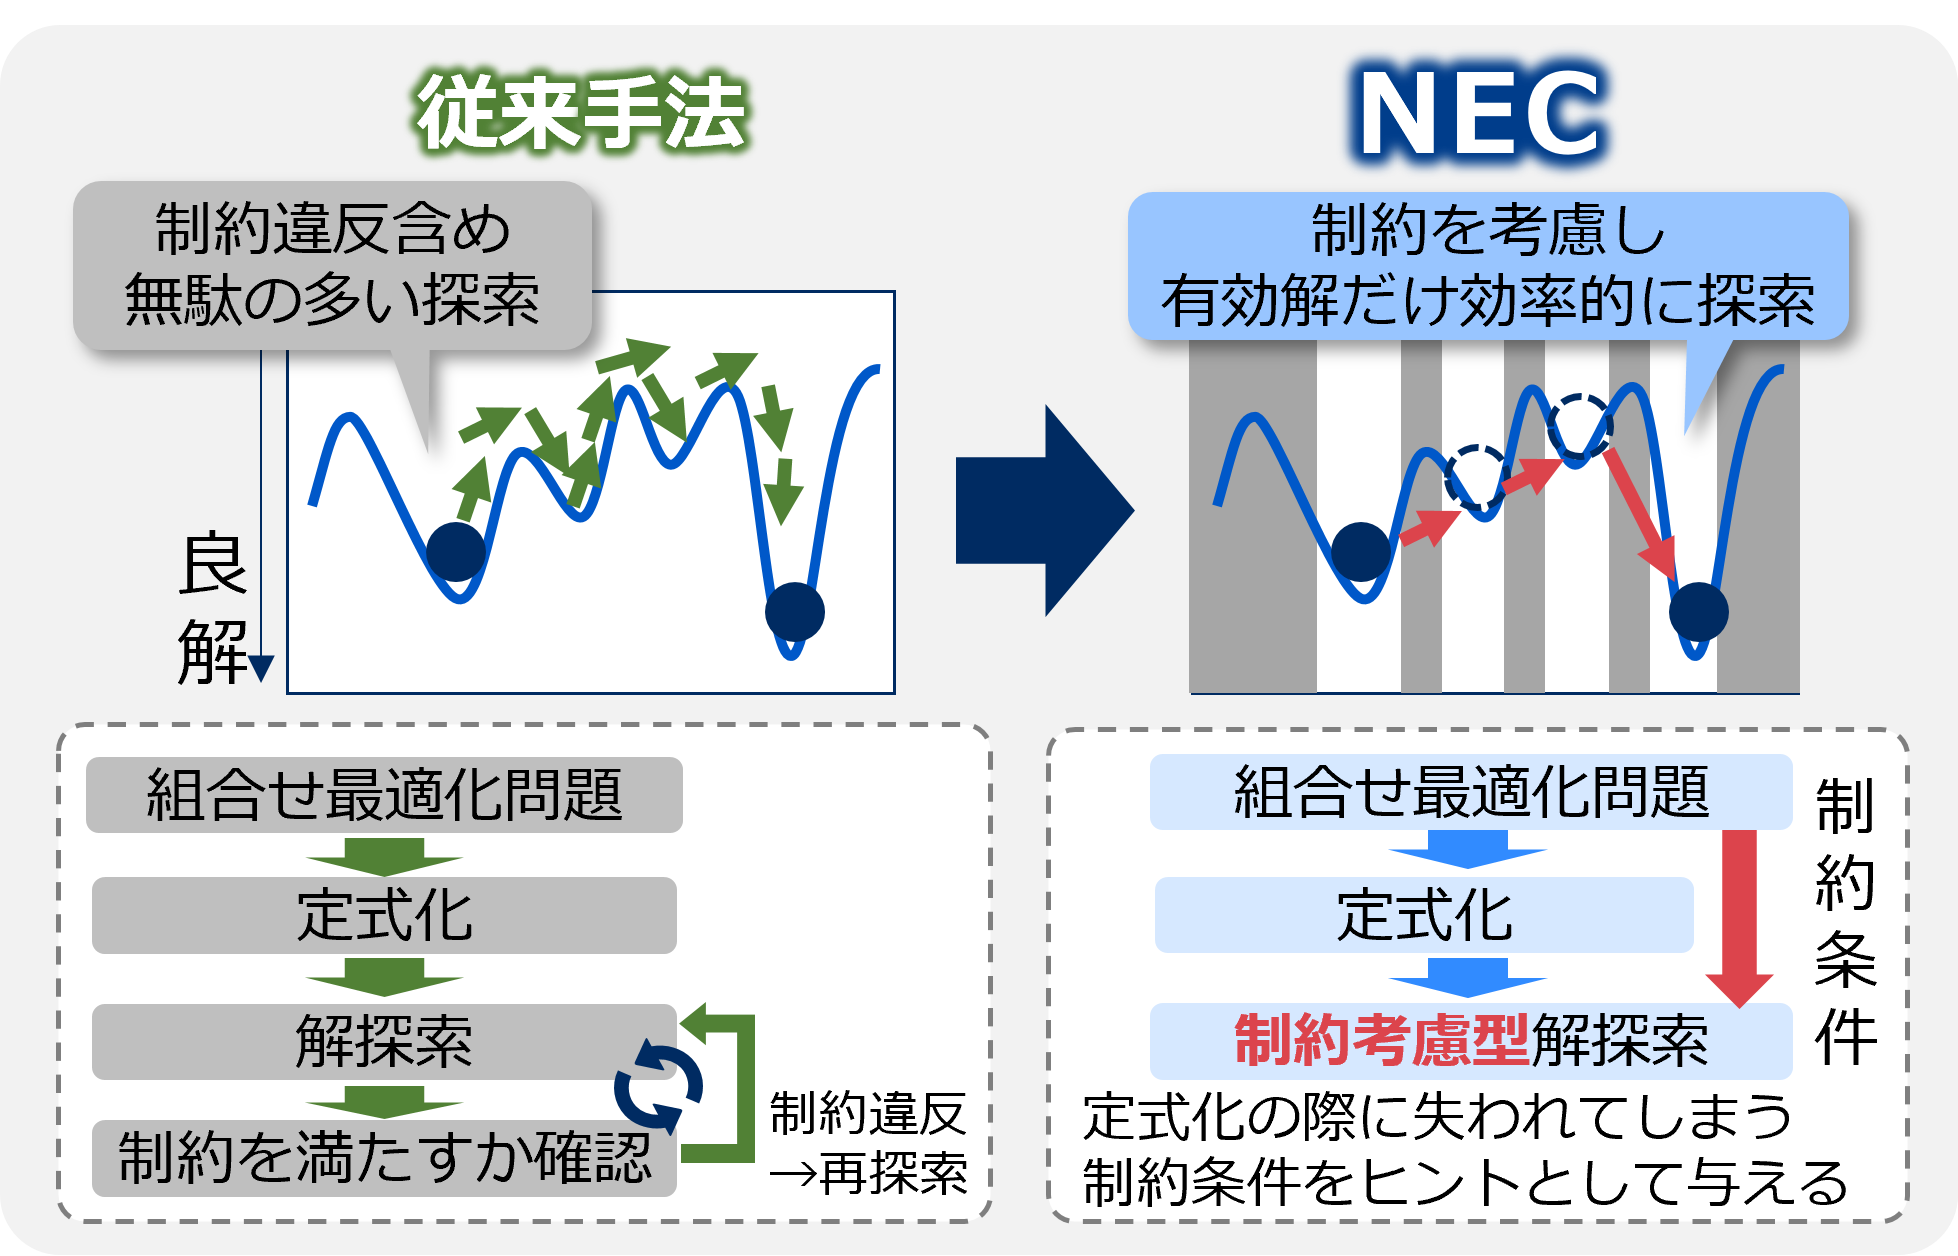
\includegraphics[bb=0 0 775 250, width=15cm]{NEC_VA_flip_option.png}
% \caption{NEC VAによる制約を考慮した探索.}
% \label{va_search}
% \end{figure}

\begin{figure}[ht]
\centering
\subfigure[従来のアニーリングによる解探索]{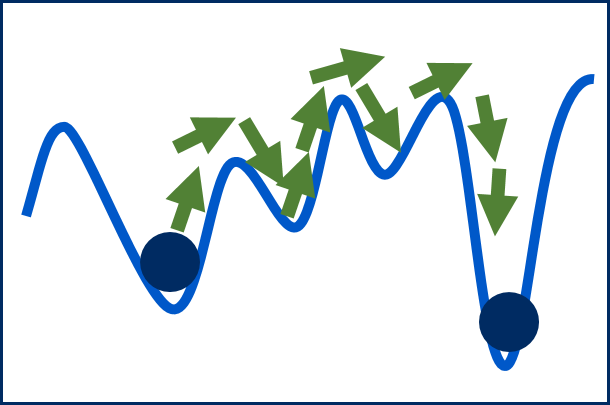
\includegraphics[bb=0 0 140 90, width=3.5cm]{normal_search.png}}
\hspace{5mm}
\subfigure[制約条件を考慮した解探索]{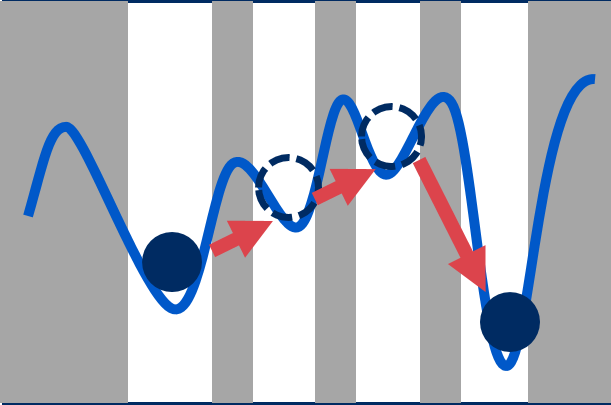
\includegraphics[bb=0 0 140 90, width=3.5cm]{va_search.png}}
\caption{制約機能を持つ擬似量子アニーリングマシンによる解探索}
\label{va_search}
\end{figure}

\begin{sourcecode}[h] % Figure環境と同様にhtbが使えます.pは使えません.
% \vspace{3mm}
\caption{制約機能の使用例}\label{code:nec_va}
\begin{lstlisting}
# 制約条件の情報を配列形式で定義
one_hot_list = [
    ['x[0][0]', 'x[0][1]', 'x[0][2]', 'x[0][3]'],
    ['x[1][0]', 'x[1][1]', 'x[1][2]', 'x[1][3]'],
    ['x[2][0]', 'x[2][1]', 'x[2][2]', 'x[2][3]'],
]

# モデル作成時に制約条件を入力
va_model = VectorAnnealing.model(qubo, offset, onehot=one_hot_list)
\end{lstlisting}
\vspace{3mm}
\end{sourcecode}

%4
\section{性能評価}

%4.1
\subsection{評価環境}
\textcolor{blue}{本評価では, 制約機能の有効性の評価のために, NEC VAを用いて制約機能を指定する場合と, 制約条件をペナルティ関数として導入する場合の比較を行う. ここで, NEC VAの制約機能を指定する場合, 探索方式の異なる二つの制約処理を選択することができる. 制約活用探索では, 外部入力された制約条件を探索時のヒント情報として活用する. 即ち近傍を選択する際に制約破壊しているスピンを1つ以上訂正することで効率的な探索を行う. 制約充足探索では, 外部入力された全ての制約条件を完全に満たす状態の中から解探索を行う. 評価では, 問題に応じてこれら二つのうち, より高い精度が得られた探索方式を採用した. また, 評価ではNEC VAをオンプレミス環境上での実行とした.} 


\textcolor{blue}{ベンチマーク問題として, 制約を含まないMaxcut, 及び異なる制約を含む4つの最適化問題(QAP, TSP, QKP, MIS)を用いる. 性能評価の指標として, 複数実行により得られるTime to Solution (TTS)を使用する. ここで, TTSはアニーリングの性能評価に一般的に用いられる指標であり, 以下の式で表される.}
\begin{equation}
{\rm{TTS}}(\tau, p_{R}) = \tau\frac{{\rm{ln}}(1-p_{R})}{{\rm{ln}}(1-p_{s}(\tau))} \label{tts_def}
\end{equation}
\textcolor{blue}{ここで, $\tau$は1回あたりの計算時間, $p_{R}$は任意に決める値であり, 目標精度の解を得る確率の閾値である. $p_{s}(\tau)$は実際にその計算時間で目標精度の解を得た正答確率である. 評価では$p_{R}=0.99$とする. ここで精度とは, 既知最適解における目的関数値からの誤差率を表す. 例えば精度1\%の場合, 最適解における目的関数値x1.01倍の目的関数値の解までを正答と見做す. 目標精度の決め方として, 本評価では各ベンチマーク問題において到達可能な最良の精度を選択した. 表\ref{table_target}に, 各ベンチマーク問題毎に設定したTTSの基準とする目標精度を示す. また, 計算の実行回数として, 全てのベンチマーク問題で10回とした.}

\newlength{\myheight}
\setlength{\myheight}{0.8cm}

\begin{table*}[htb]
\centering
  \caption{各疑似量子アニーリングマシンの仕様}
    \begin{tabular}{|c||c|c|c|c}
      \hline
      \parbox[c][\myheight][c]{0cm}{}
      & {NEC VA} & {Fujitsu DA} & {Fixstars Amplify AE}\\ \hline \hline
      求解方式 & Simulated Annealing & MCMC Parallel Tempering & Simulated Annealing\\ \hline
      利用形態 & オンプレミス & クラウド & クラウド\\ \hline
      動作プラットフォーム & X86 CPU & GPU & Nvidia A100\\ \hline
      最大ビット/スピン数 & 10,0000+ & 10,0000+ & 262,144\\ \hline
      ビット階調 & 32bits/64bits & 64bits & 32bits/64bits\\ \hline
      制約処理技術 & 1hot & 2way-1hot  & -\\ 
      {} & 不等式制約 & 不等式制約 & {}\\ \hline
  \end{tabular}
\label{table_spec}
\end{table*}

% \begin{table}[tb]
% \centering
%   \caption{各ベンチマーク問題における制約重みの設定}
%     \begin{tabular}{|c||c|c|c}
%       \hline
%       \parbox[c][\myheight][c]{0cm}{}
%       & \parbox{10em}{Fixstars Amplify AE} & {NEC VA}\\ \hline \hline
%       TSP & $0.1\alpha\sim0.5\alpha\,(\alpha={\rm Max}(d_{i,j}))$ & $0.04\alpha\sim0.05\alpha$\\ \hline
%       QAP & $\beta\sim20\beta\,(\beta={\rm Max}(f_{i,j}d_{k,l}))$ & \multirow{3}{*}{-}\\
%        \cline{1-1} \cline{2-2}
%       QKP & \multirow{2}{*}{1.0} & \\
%       \cline{1-1}
%       MIS & & \\ \hline
%   \end{tabular}
% \label{table_weight}
% \end{table}

\begin{table}[tb]
\centering
  \caption{各ベンチマーク問題におけるTTSの目標精度}
    \begin{tabular}{|c||c|c|c|}
      \hline
      \multirow{2}{*}{Maxcut} & G65 & G72 & G81\\
      \cline{2-2} \cline{3-3} \cline{4-4}
                            & \multicolumn{3}{|c|}{0.2\%}\\ \hline
      \multirow{2}{*}{TSP} & ch150 & kroA200 & pr226\\
      \cline{2-2} \cline{3-3} \cline{4-4}
                              & 1\% & 5\% & 10\%\\ \hline
      \multirow{2}{*}{QAP} & tai80b & tai100b & tai150b\\
      \cline{2-2} \cline{3-3} \cline{4-4}
                            & \multicolumn{3}{|c|}{1\%}\\ \hline
      \multirow{2}{*}{QKP} & jeu\_100\_50\_1 & jeu\_200\_50\_1 & jeu\_300\_50\_1\\
      \cline{2-2} \cline{3-3} \cline{4-4}
                            & \multicolumn{3}{|c|}{最適解}\\ \hline
      \multirow{2}{*}{MIS} & frb\_53\_24\_1 & frb\_59\_26\_1 & frb\_100\_40\\
      \cline{2-2} \cline{3-3} \cline{4-4}
                            & \multicolumn{3}{|c|}{最適解}\\ \hline
    \end{tabular}
\label{table_target}
\end{table}

%4.2
\subsection{実験結果}

%4.2.1
\subsubsection{制約を含まないMaxcutによる評価}
\textcolor{blue}{図\ref{TTS_Maxcut_VA}に, MaxcutによるTTSの評価結果を示す. データセットとして, Gset\cite{gset}のうち3つのインスタンスを用いた. X軸は各インスタンス名を示しており, インスタンス名の数値が大きいほど変数量が大きい. Y軸は各インスタンスにおけるTTSを示しており, 値が小さいほど性能が高いことを表す. 図\ref{TTS_Maxcut_VA}より, 問題規模の増大に伴いTTSが増加していく傾向が見られる. この要因を考察するために, 解精度分布による評価を行う. 図\ref{Cost_Maxcut_VA}に, 図\ref{TTS_Maxcut_VA}と同実行により得られた解精度分布を示す. 図\ref{Cost_Maxcut_VA}より, 問題規模が増大した場合でも解精度は大きく変化しないことが分かる. 従って, TTSの悪化要因が問題規模の増加に伴う実行時間の増加に起因することが分かる. 実行時間が増加する要因として, 問題規模の増大とともに探索空間が増大し, 低エネルギー解へ到達するまでの時間が増加したためだと考えられる.}

\begin{figure}[t]
\centering
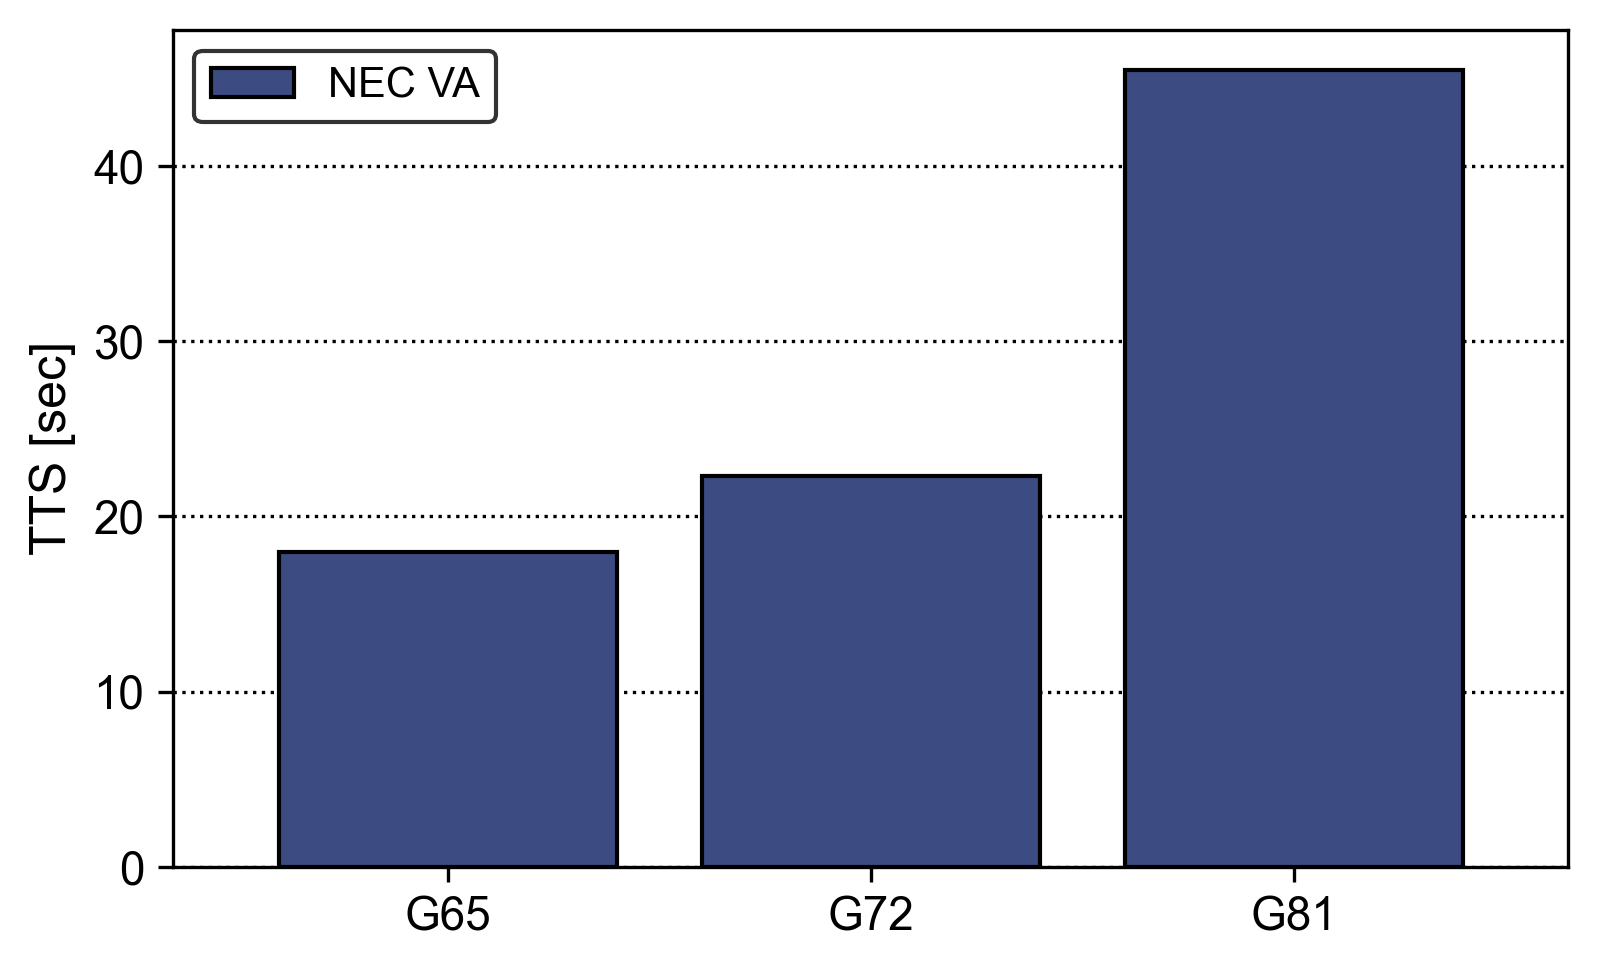
\includegraphics[bb=0 0 700 230, width=15cm]{TTS_Maxcut_VA.png}
\caption{NEC VAによるTTSの比較(Maxcut).}
\label{TTS_Maxcut_VA}
\end{figure}

\begin{figure}[t]
\centering
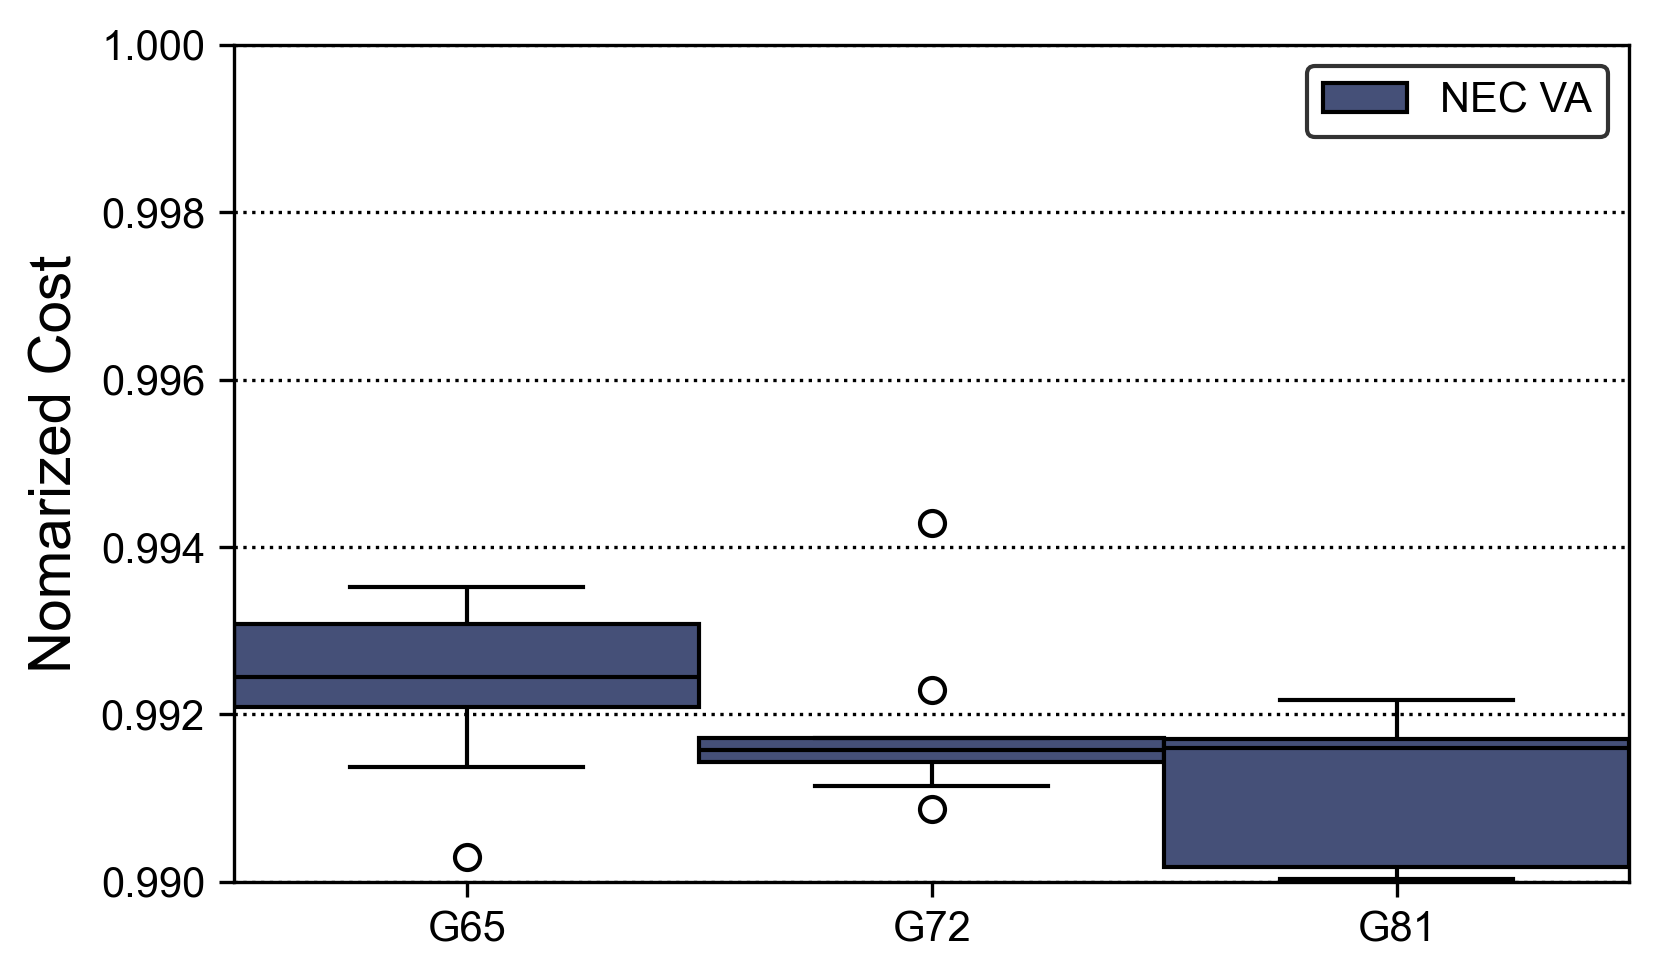
\includegraphics[bb=0 0 700 230, width=15cm]{Cost_Maxcut_VA.png}
\caption{NEC VAによる解精度の比較(Maxcut).}
\label{Cost_Maxcut_VA}
\end{figure}

%4.2.2
\subsubsection{ワンホット制約を持つTSP, QAPによる評価}
\textcolor{blue}{図\ref{TTS_TSP_VA}に, TSPによるTTSの評価結果を示す. データセットとして, TSPLIB\cite{tsplib}のうち3つのインスタンスを使用した. X軸は各インスタンス名を示しており, インスタンス名の数値が大きいほど変数量が大きい. Y軸は各インスタンスにおけるTTSを示している. また, 同図においてTTSが表示されていない場合, そのインスタンスにおいて目標精度の解が得られなかったことを表す.}

\textcolor{blue}{図\ref{TTS_TSP_VA}に示す通り, TSPにおいて制約条件をペナルティ関数として導入する場合(penalty function), 測定した全ての実行において目標精度を満たす解が得られていない. また図\ref{Cost_TSP_VA}に, 同実行により得られた解精度分布を示す. 図\ref{Cost_TSP_VA}より, 制約条件をペナルティ関数として導入する場合, 制約機能を指定する場合(external constraint)と比較して全インスタンスで解精度が悪く, 問題規模の増大に伴う解精度の悪化も大きいことが分かる. これは, 変数量の増加に伴い解空間が増大したことに加えて, ペナルティ関数を導入したことにより探索空間における有効解の割合が大きく減少し, 低エネルギー解への遷移が難しくなったためだと考えられる. 一方, 制約機能を使用することで, 制約条件を満たす有効解を効率的に探索できるため, 大規模においても高い解精度を維持したと考えられる.}

% また同図において, NEC VAの制約処理方式の違いによる解精度を比較すると, 制約活用探索よりも制約充足探索の方が高い解精度に到達していることが分かる. この要因として, 制約充足探索では制約条件を満たした解のみを探索するのに対して, 制約活用探索では解探索の途中で制約違反状態を経由するため, 制約活用探索ではエネルギーが低下した段階での遷移が活発になり高精度な解に収束しやすくなったと考えられる.

% \textcolor{blue}{二つの探索について, まず制約活用探索のみ目的関数にペナルティ項を含めるという違いがある. ペナルティ項は目的関数の重みに対し係数が大きい場合にQUBOのエネルギー地形を複雑化して局所解へトラップしやすくなる一方, 係数が小さい場合エネルギー地形を平易化して最適解への収束を補助する場合もあると考えらえる. 二つ目の違いとして制約充足探索では制約を満たした解のみ探索するのに対し, 制約活用探索では制約違反状態も経由し制約違反するスピンが徐々に少なくなるように補助的な遷移を加えつつ探索する違いがある. 以上を踏まえ結果を見ると制約活用探索はTSPにおいて小さい係数のペナルティ項で制約を満たせているので, 制約充足探索と比較してエネルギーが下がった段階での遷移が活発になり良い解に収束したと考えられる.}

\begin{figure}[th]
\centering
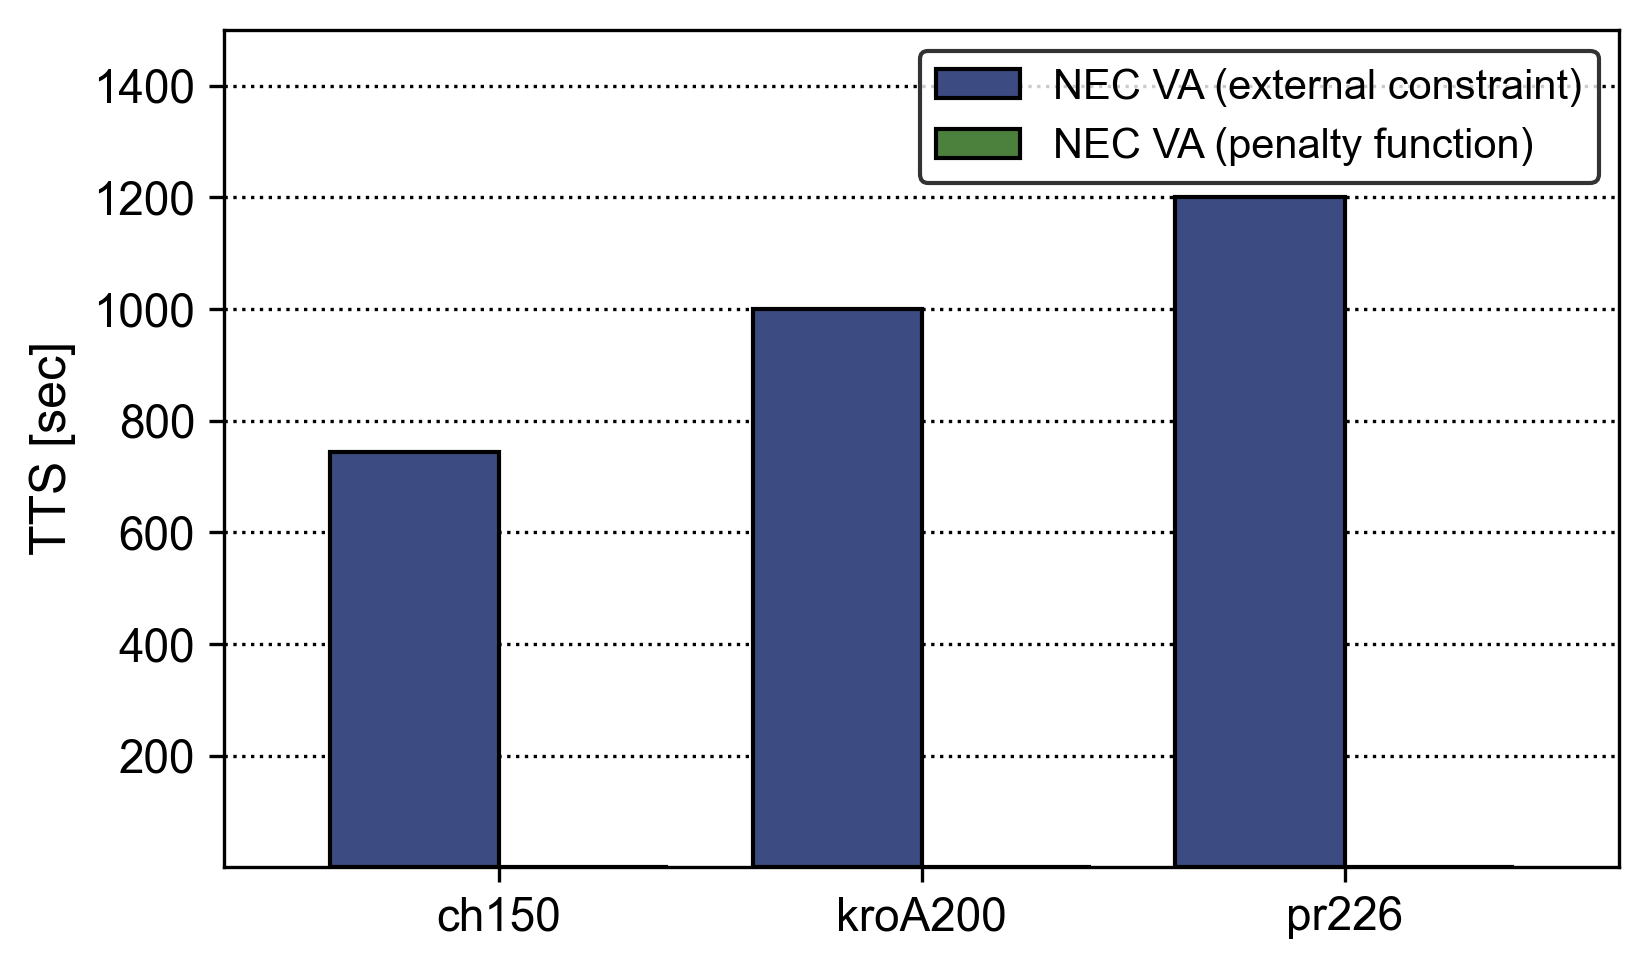
\includegraphics[bb=0 0 700 230, width=15cm]{TTS_TSP_VA.png}
\caption{NEC VAによるTTSの比較(TSP).}
\label{TTS_TSP_VA}
\end{figure}

\begin{figure}[th]
\centering
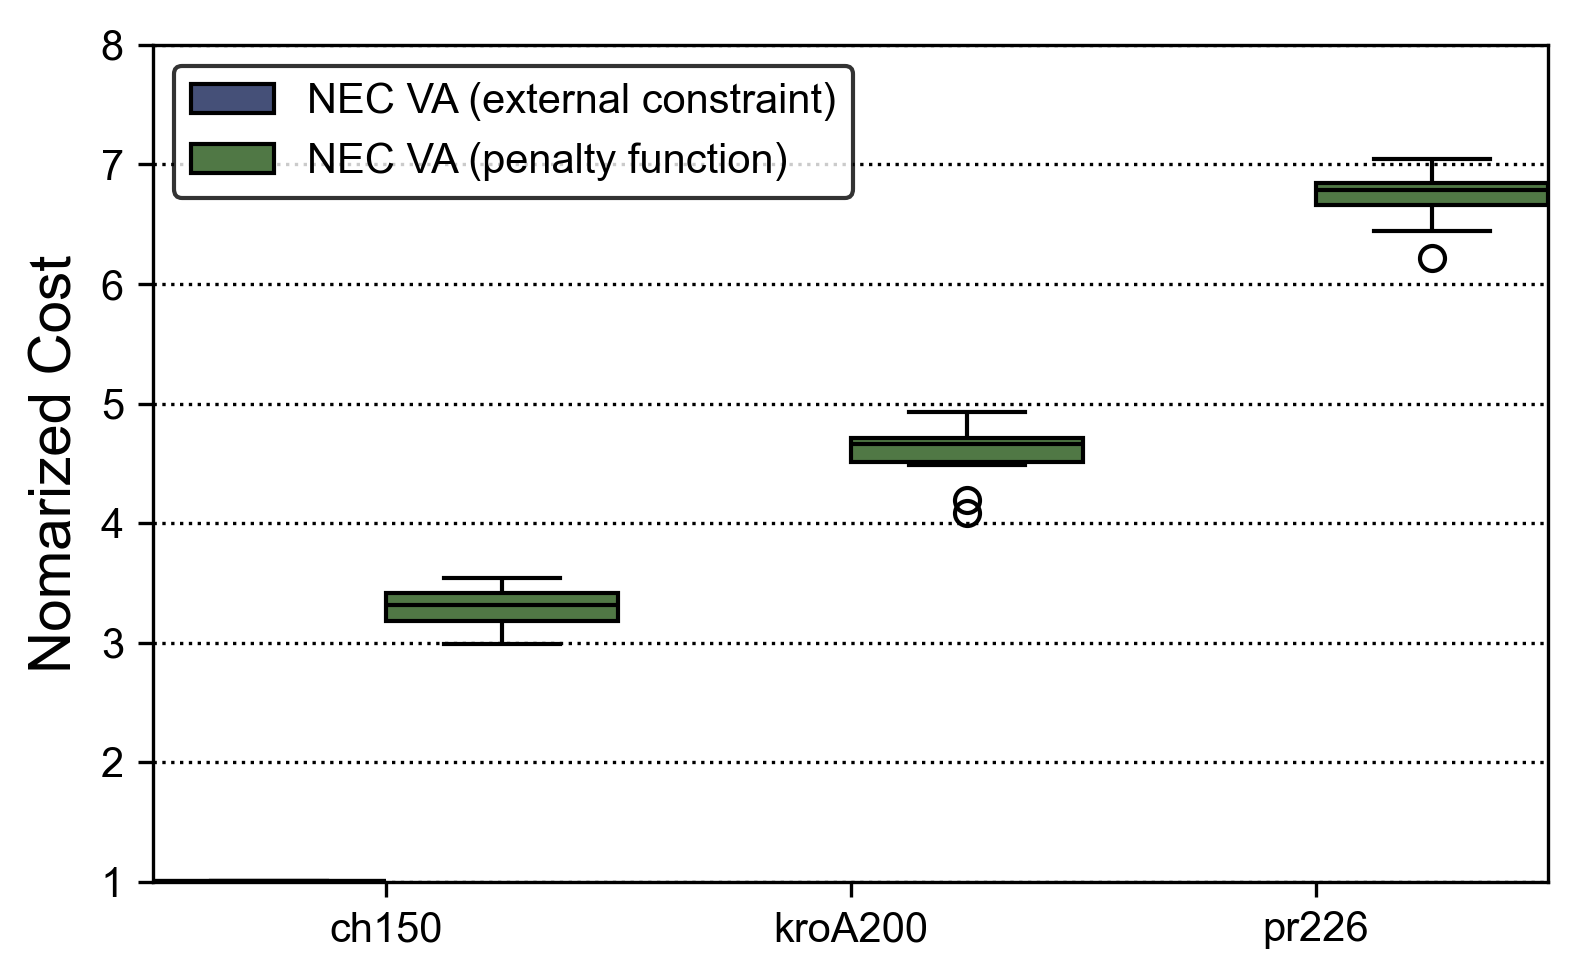
\includegraphics[bb=0 0 700 230, width=15cm]{Cost_TSP_VA.png}
\caption{NEC VAによる解精度の比較(TSP).}
\label{Cost_TSP_VA}
\end{figure}

\textcolor{blue}{図\ref{TTS_QAP}に, QAPによるTTSの評価結果を示す. データセットとして, QAPLIB\cite{qaplib}のうち3つのインスタンスを用いた. X軸は各インスタンス名を示しており, インスタンス名の数値が大きいほど変数量が大きい. Y軸は各インスタンスにおけるTTSを示している. }

\textcolor{blue}{図\ref{TTS_QAP_VA}に示す通り, QAPにおいて制約条件をペナルティ関数として導入する場合, 測定した全ての実行において目標精度を満たす解が得られていない. また図\ref{Cost_QAP_VA}に, 同実行により得られた解精度分布を示す. 図\ref{Cost_QAP_VA}より, 制約条件をペナルティ関数として導入する場合, 制約機能を指定する場合と比較して全インスタンスで解精度が悪いことが分かる. これは, TSPと同様に, ペナルティ関数を導入したことにより, 探索空間における有効解の割合が減少し, 低エネルギー解への遷移が難しくなったためだと考えられる. 
また, QAPにおいて制約条件を満たす有効解を得るためには, 問題規模の増大に応じてペナルティ関数に掛かる重みを大きく設定する必要がある\cite{qaplib}. これにより, 大規模問題ではペナルティ関数によるエネルギー関数の変動が大きくなり, 探索精度により影響を与えたと考えられる. 一方, 制約機能を指定することにより, 探索空間を限定できる上, 大規模でもペナルティ関数の影響を受けることなく効率的に探索できるため, 高い解精度に到達できたと考えられる. }

% また同図において, NEC VAの制約処理方式の違いによる解精度を比較すると, TSPとは異なり, 制約活用探索よりも制約充足探索の方が高い解精度に到達していることが分かる. この要因として, 制約活用探索では制約のペナルティ関数を含める必要があり, 前述の通りQAPではこのペナルティの重みがTSPと比較して大きな値となるため, 制約充足探索と比較して探索空間のランドスケープが複雑になり, 早い段階で局所解に捕捉されたことが結果に影響したと考えられる.

% \textcolor{blue}{TSPの考察で見たように制約活用探索はペナルティ項を追加する必要があるが, QAPの場合はこの係数を比較的大きくしなければ制約を満たせない. 理由として, TSPに対し重み係数の分散が大きく項も多いので, 制約破壊時のエネルギー変化が大きくなりやすくそれに合わせた係数のペナルティ項が必要になることが考えられる. そのためペナルティ項がエネルギー地形を複雑化し, 制約充足探索よりも早い段階で局所解にトラップしたことで悪い結果になったと考えられる. また制約充足探索においてもTSPに対しQAPでは解精度が良い. 制約は同じツーウェイワンホットであるため目的関数の差, 例えばQUBO行列の密度や重み係数の分散の違いが影響している可能性がある. }

\begin{figure}[th]
\centering
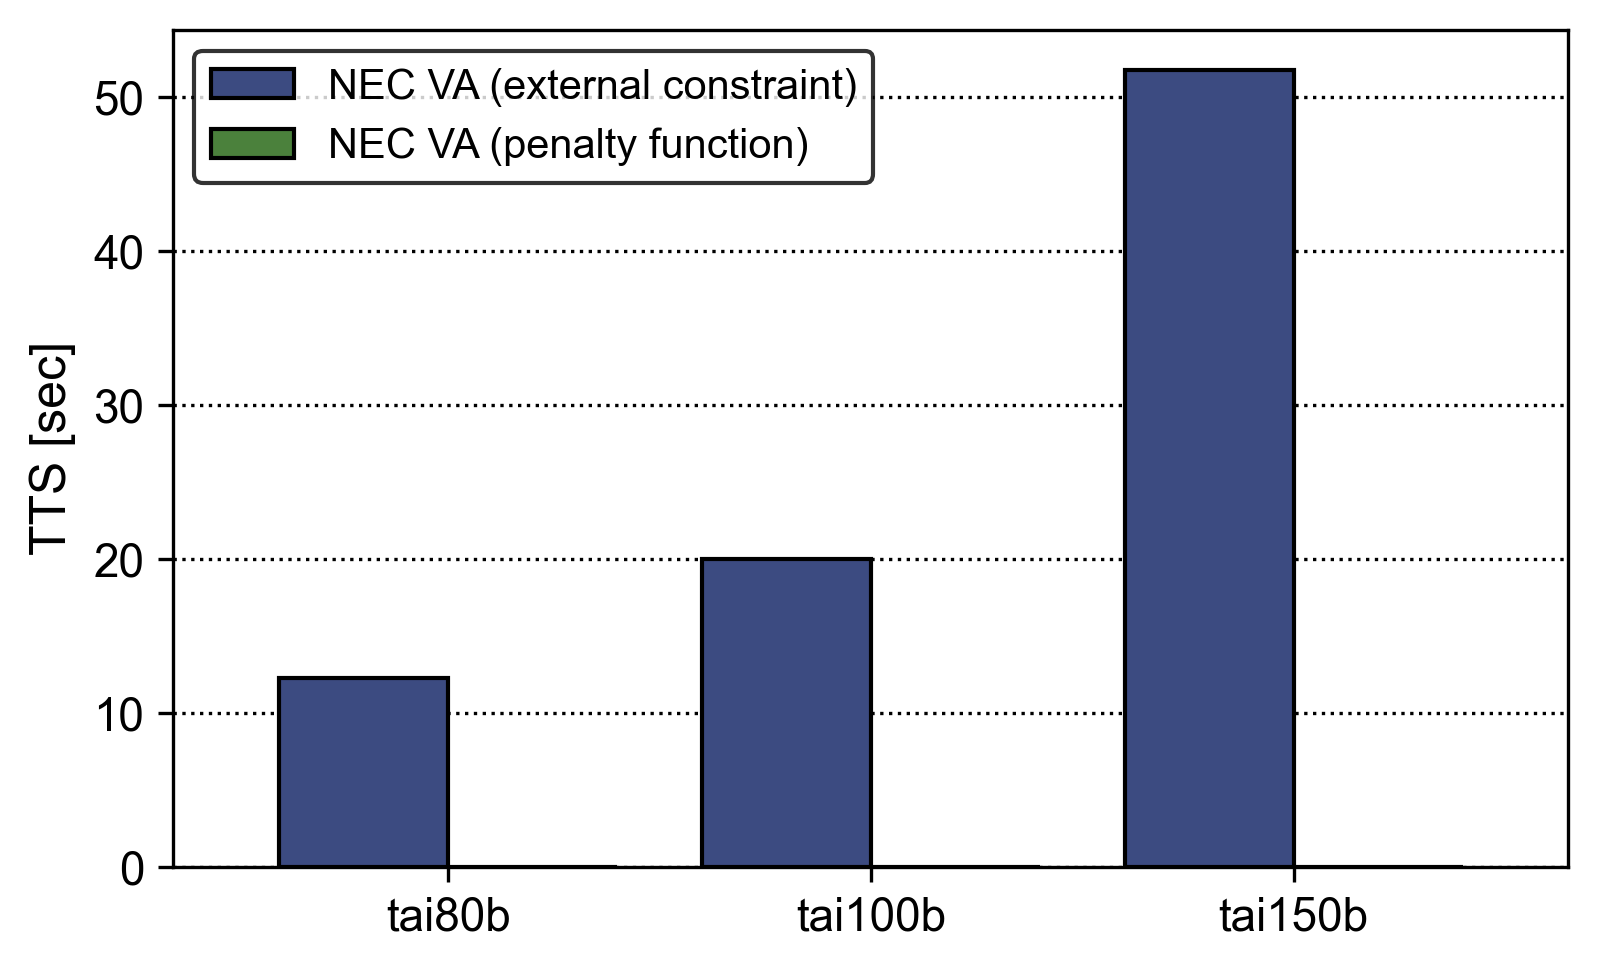
\includegraphics[bb=0 0 700 230, width=15cm]{TTS_QAP_VA.png}
\caption{NEC VAによるTTSの比較(QAP).}
\label{TTS_QAP_VA}
\end{figure}

\begin{figure}[th]
\centering
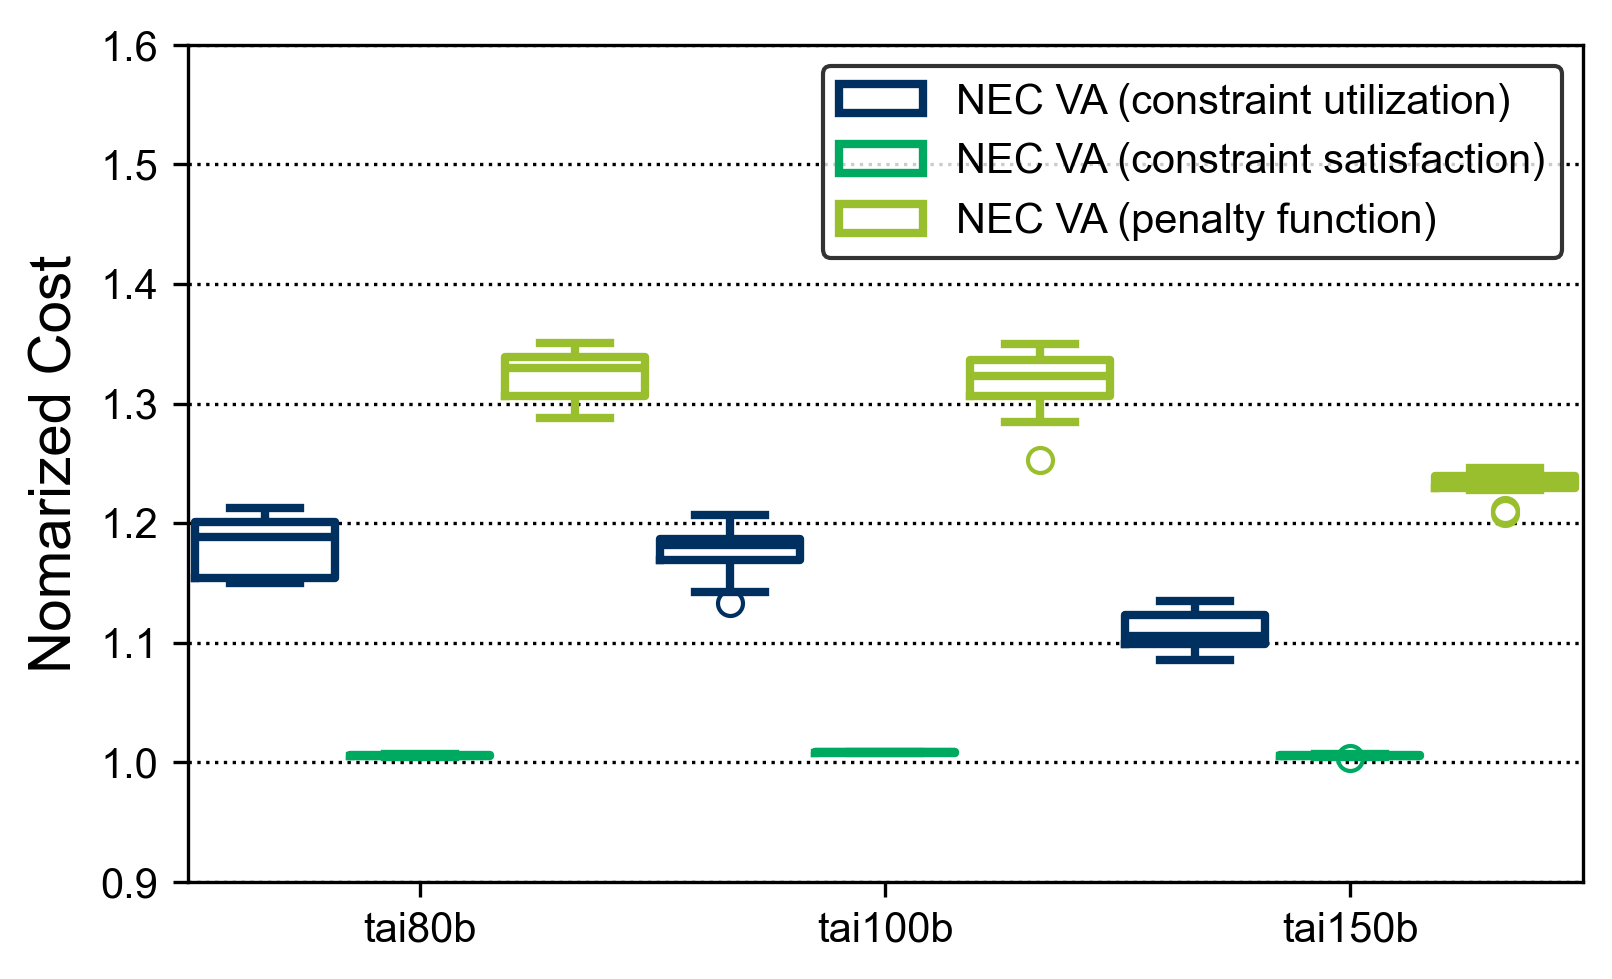
\includegraphics[bb=0 0 700 230, width=15cm]{Cost_QAP_VA.png}
\caption{NEC VAによる解精度の比較(QAP).}
\label{Cost_QAP_VA}
\end{figure}

%4.2.3
\subsubsection{不等式制約を持つQKPによる評価}
\textcolor{blue}{図\ref{TTS_QKP_VA}に, QKPによるTTSの評価結果を示す. データセットとして, 先行研究\cite{qkplib}で作成されたQKPインスタンスのうち3つのインスタンスを用いた. 図\ref{TTS_QKP_VA}のX軸は各インスタンス名を示しており, インスタンス名に含まれる3つの数字は左からそれぞれ, 変数量, QUBOの結合密度, 及びインスタンスの種類を示している. Y軸は各インスタンスにおけるTTSを示している. }

\textcolor{blue}{図\ref{TTS_QKP_VA}に示す通り, QKPにおいて制約条件をペナルティ関数として導入する場合, 測定した全ての実行において目標精度を満たす解が得られていない. また図\ref{Cost_QKP_VA}に, 同実行により得られた解精度分布を示す. 図\ref{Cost_QKP_VA}より, 不等式制約をペナルティ関数として導入する場合, 制約機能を指定する場合と比較して全インスタンスで解精度が悪いことが分かる. この要因として, 不等式制約のペナルティ関数を導入する場合, エネルギー関数の変動に加えて, ペナルティ関数の導入過程で補助変数が追加されたことにより解空間が増加し, 探索精度に影響を与えたと考えられる. 一方, 制約機能を使用した場合, エネルギー関数にはペナルティ関数及び補助変数が含まれず, これらの影響を回避できたため, 高い解精度まで到達できたと考えられる.}

\begin{figure}[t]
\centering
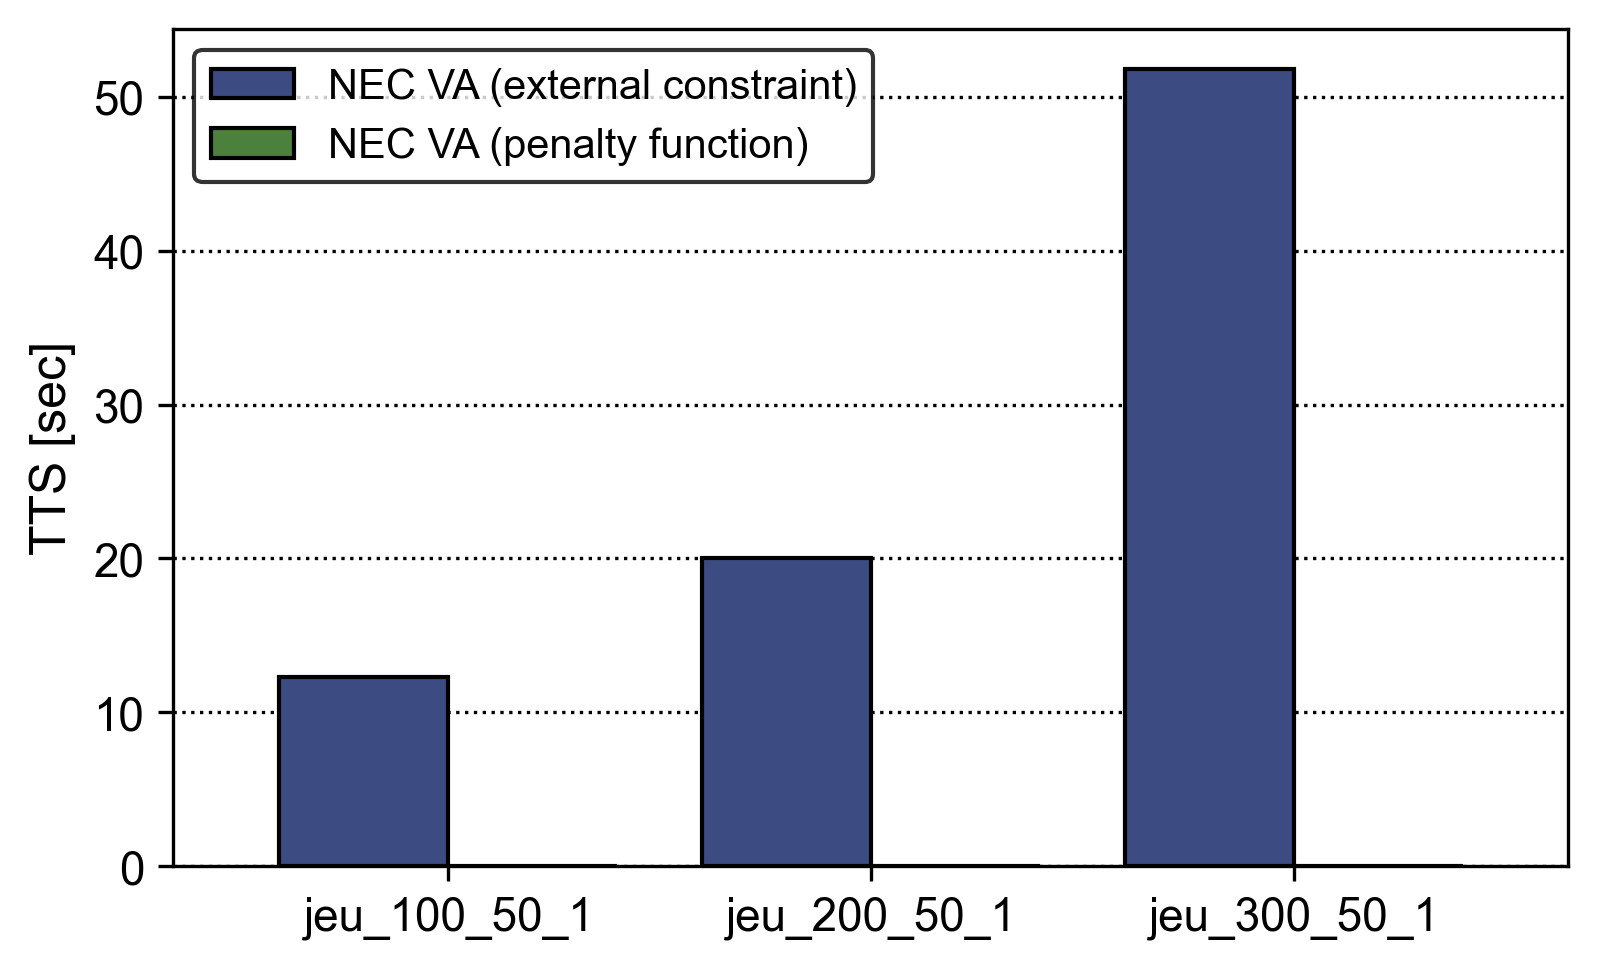
\includegraphics[bb=0 0 700 230, width=15cm]{TTS_QKP_VA.png}
\caption{NEC VAによるTTSの比較(QKP).}
\label{TTS_QKP_VA}
\end{figure}

\begin{figure}[t]
\centering
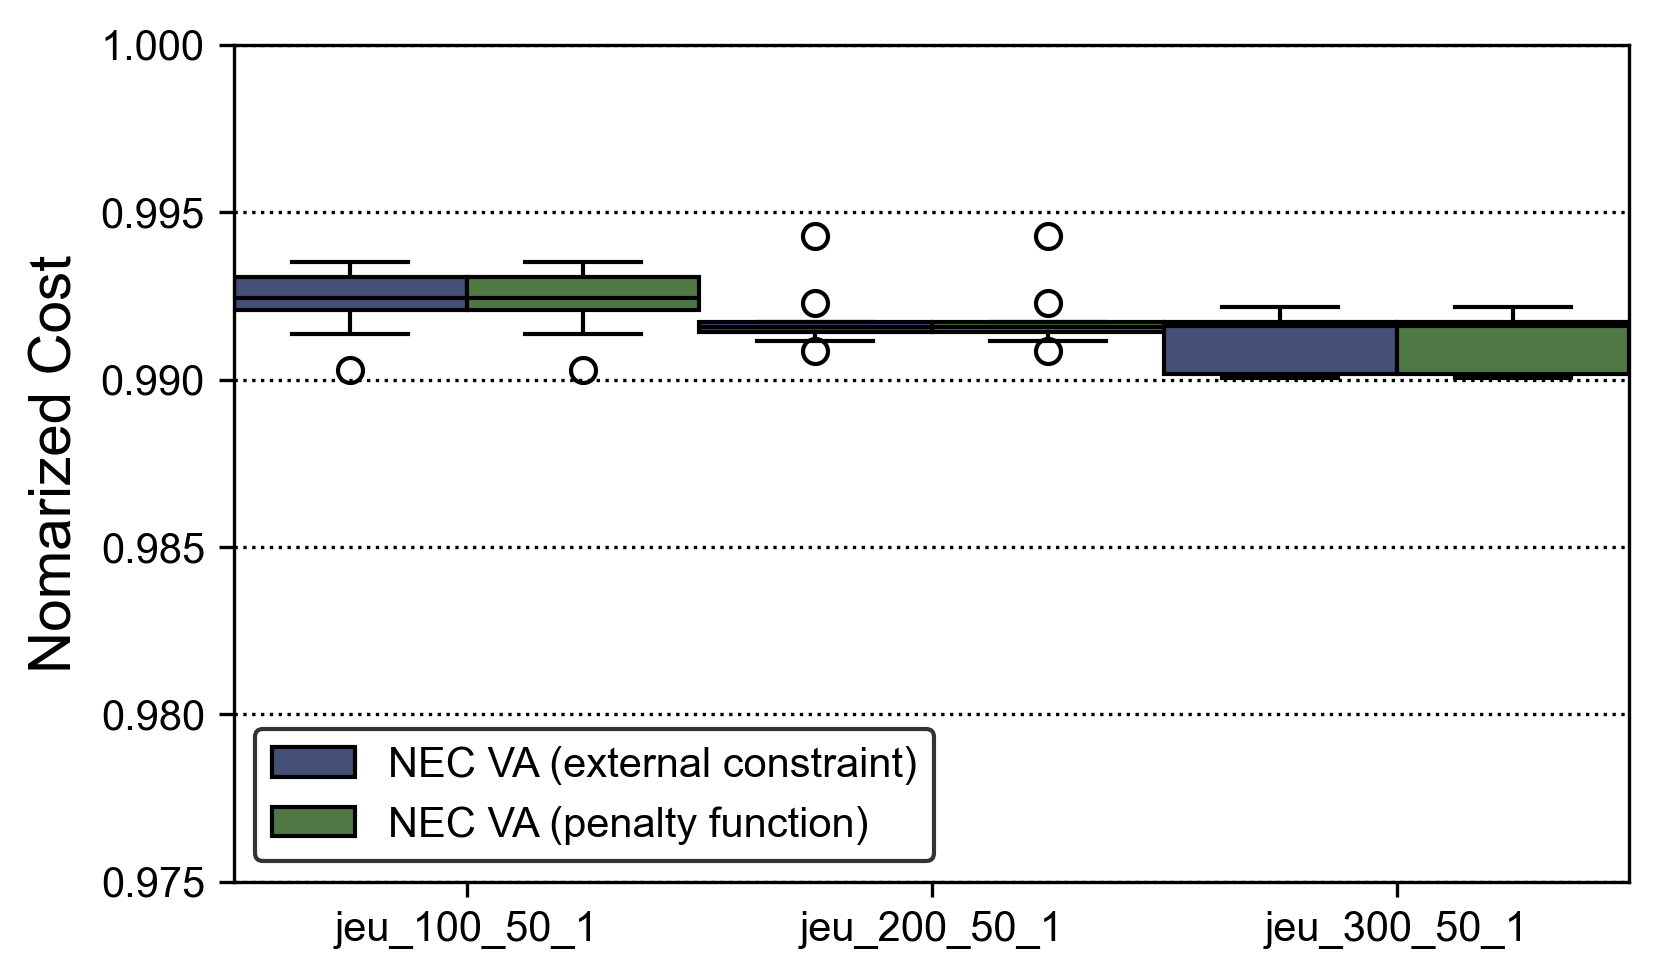
\includegraphics[bb=0 0 700 230, width=15cm]{Cost_QKP_VA.png}
\caption{擬似量子アニーリングマシンによる解精度の比較(QKP).}
\label{Cost_QKP_VA}
\end{figure}

%4.2.4
\subsubsection{禁止ペア制約を持つMISによる評価}
\textcolor{blue}{図\ref{TTS_MIS_VA}に, MISによるTTSの評価結果を示す. データセットとして, BHOSLIB\cite{mislib}のうち3つのインスタンスを用いた. 図\ref{TTS_MIS_VA}のX軸は各インスタンスを示しており, 各インスタンス名のfrbの直後の数値が大きいほど問題の変数量が大きいことを示している. Y軸は各インスタンスにおけるTTSを示している.}

\textcolor{blue}{図\ref{Cost_MIS_VA}に示す通り, MISでは制約機能の有無によらず, 全インスタンスで目標精度を満たす解が得られており, この時のTTSは禁止ペア制約をペナルティ関数として導入する場合の方が小さいことが分かる. また図\ref{Cost_MIS_VA}に, 同実行により得られた解精度分布を示す. 図\ref{Cost_MIS_VA}より, MISでは制約機能を使用する場合, 及びペナルティ関数を含める場合ともに, 全インスタンスで最適解に収束していることが分かる. 従って, 図\ref{TTS_MIS}におけるTTSの差は, 制約機能を使用する場合とペナルティ関数を含める場合による実行時間の差に起因することが分かる. 制約条件をペナルティ関数として導入する場合に高い精度を実現できる要因として, バイナリ変数の積で構成される禁止ペア制約は二次式であるQUBO表現と相性が良く, ペナルティ関数を追加することによるエネルギー関数の変動が比較的小さいと考えられる. これにより, ペナルティ関数を含める場合でも高い求解精度を発揮できたと考えられる. また, 制約機能を指定する場合に実行時間が長くなる要因として, 外部指定された制約条件を探索時に考慮する処理が加わる分, 一探索当たりに要する実行時間が長くなったことが影響したと考えられる.}

\begin{figure}[ht]
\centering
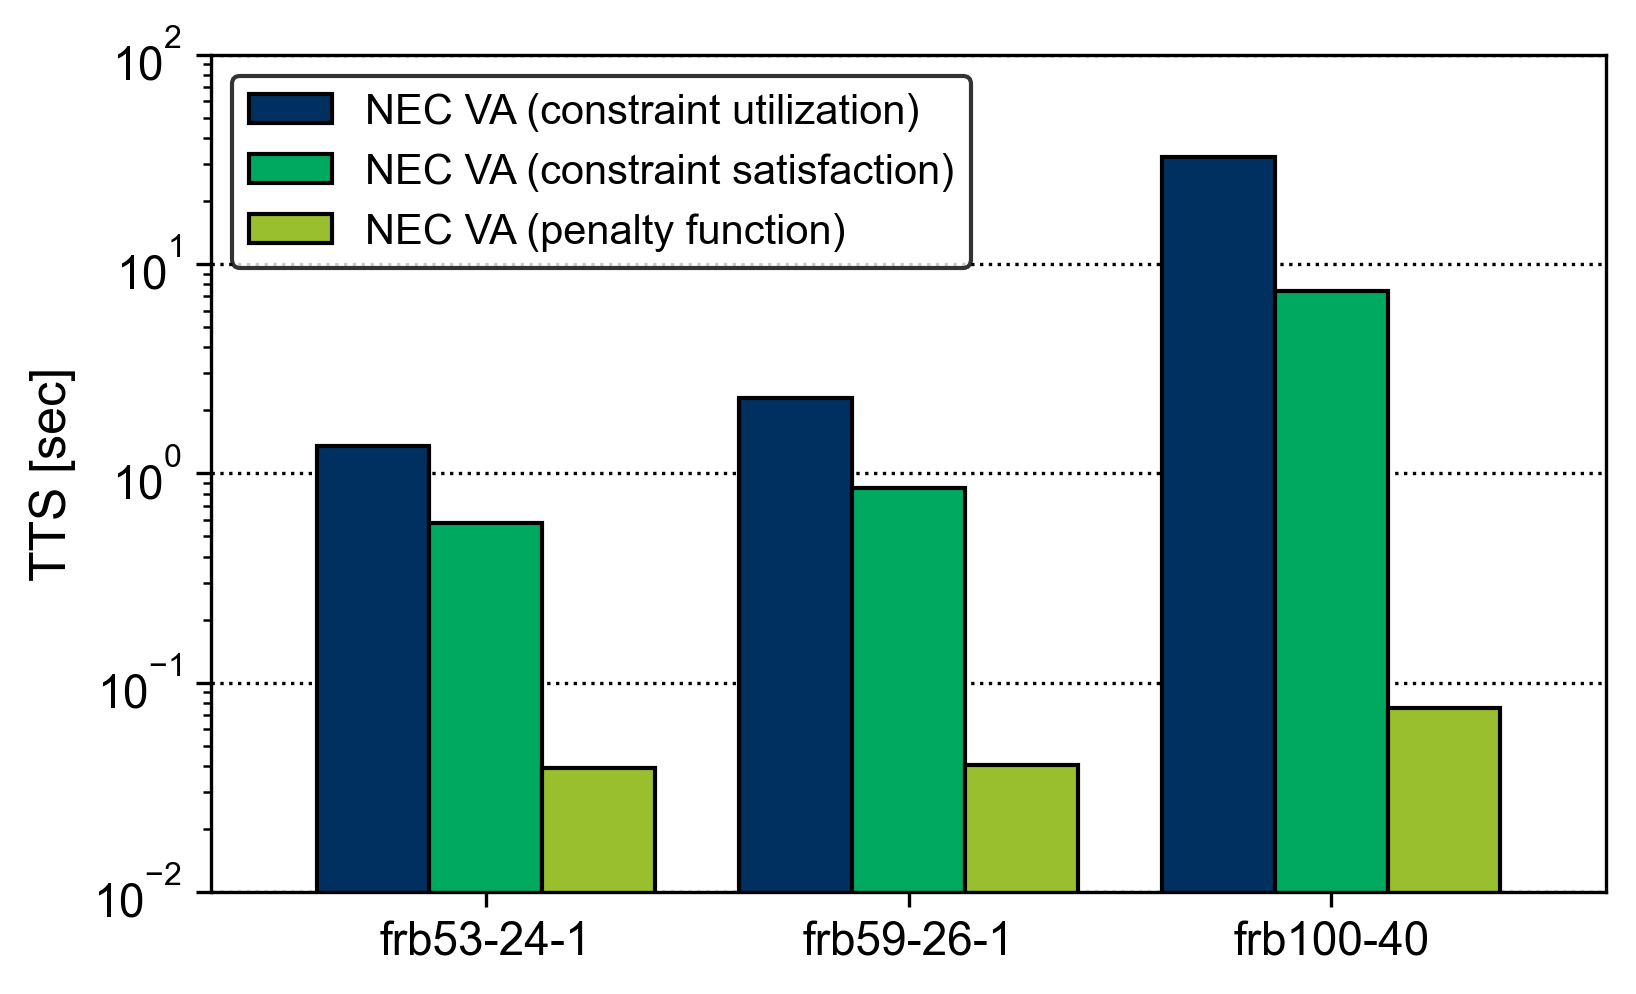
\includegraphics[bb=0 0 700 230, width=15cm]{TTS_MIS_VA.png}
\caption{NEC VAによるTTSの比較(MIS).}
\label{TTS_MIS_VA}
\end{figure}

\begin{figure}[ht]
\centering
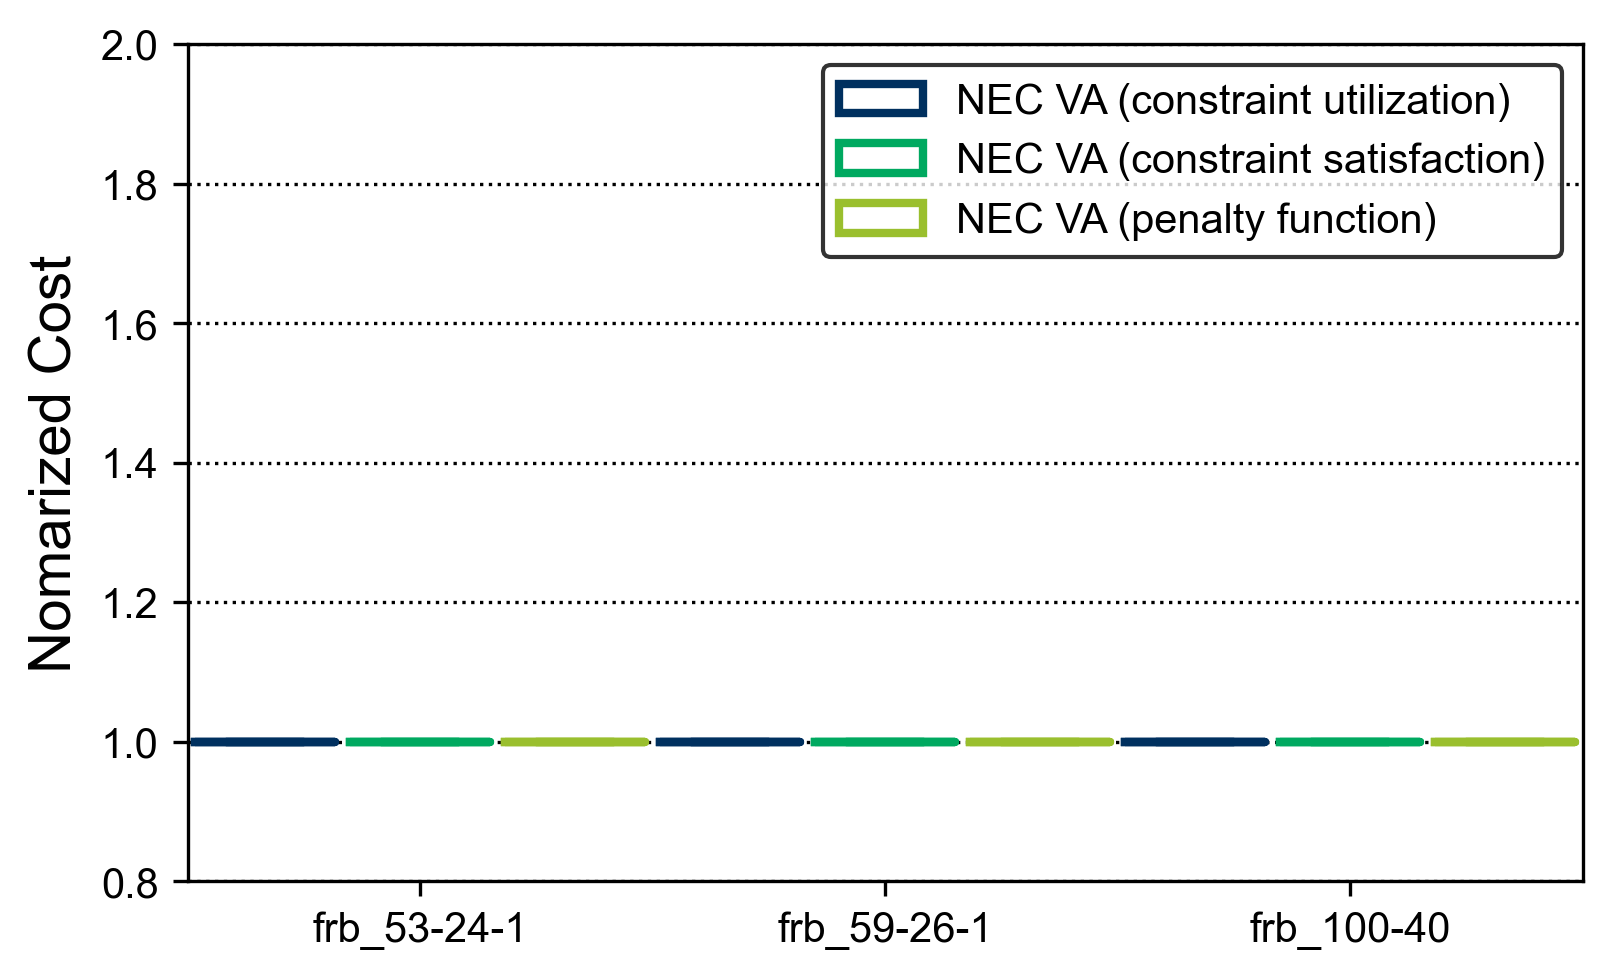
\includegraphics[bb=0 0 700 230, width=15cm]{Cost_MIS_VA.png}
\caption{NEC VAによる解精度の比較(MIS).}
\label{Cost_MIS_VA}
\end{figure}

\subsection{擬似量子アニーリングマシンによる検証}
\textcolor{blue}{本節では, 擬似量子アニーリングマシンの制約機能の有効性を確認するために, NEC VA, Fujitsu DA, Fixstars Amplify AEを用いて検証を行う. 本検証において, NEC VA, Fujitsu DAでは制約機能を指定し, Fixstars Amplify AEでは制約条件をペナルティ関数として導入する. 性能の指標として, 4.2節と同様に, TTS及び解精度を用いる. 検証に用いたTTSの目標精度を表\ref{table_target2}に示す. また, 計算の実行回数として, NEC VA, Fixstars Amplify AEでは10回, Fujitsu DAでは最大5回とした.}

\begin{table}[th]
\centering
  \caption{各ベンチマーク問題におけるTTSの目標精度}
    \begin{tabular}{|c||c|c|c|}
      \hline
      \multirow{2}{*}{Maxcut} & G65 & G72 & G81\\
      \cline{2-2} \cline{3-3} \cline{4-4}
                            & \multicolumn{3}{|c|}{1\%}\\ \hline
      \multirow{2}{*}{TSP} & ch150 & kroA200 & pr226\\
      \cline{2-2} \cline{3-3} \cline{4-4}
                              & 5\% & 6\% & 20\%\\ \hline
      \multirow{2}{*}{QAP} & tai80b & tai100b & tai150b\\
      \cline{2-2} \cline{3-3} \cline{4-4}
                            & \multicolumn{3}{|c|}{1\%}\\ \hline
      \multirow{2}{*}{QKP} & jeu\_100\_50\_1 & jeu\_200\_50\_1 & jeu\_300\_50\_1\\
      \cline{2-2} \cline{3-3} \cline{4-4}
                            & \multicolumn{3}{|c|}{最適解}\\ \hline
      \multirow{2}{*}{MIS} & frb\_53\_24\_1 & frb\_59\_26\_1 & frb\_100\_40\\
      \cline{2-2} \cline{3-3} \cline{4-4}
                            & \multicolumn{3}{|c|}{最適解}\\ \hline
    \end{tabular}
\label{table_target2}
\end{table}

%4.2.1
\subsubsection{制約を含まないMaxcutによる評価}
\textcolor{blue}{図\ref{Maxcut_TTS}に, MaxcutによるTTSの結果を示す. 図\ref{Maxcut_speed_vs_const}より, 各擬似量子アニーリングマシンにおいて, 問題規模の増大とともにTTSが大きくなる傾向が見られる. また図\ref{Maxcut_speed_vs_const}に, 同実行により得られた解精度分布を示す. 図\ref{Maxcut_speed_vs_const}より, Maxcutでは全ての擬似量子アニーリングマシンにおいて目標精度の解に到達していることが分かる. これにより, 制約条件を含まないMaxcutでは, 擬似量子アニーリングマシンに制約機能の有無によらず, 同等の解精度を実現できることが分かる.}


\begin{figure}[ht]
\centering
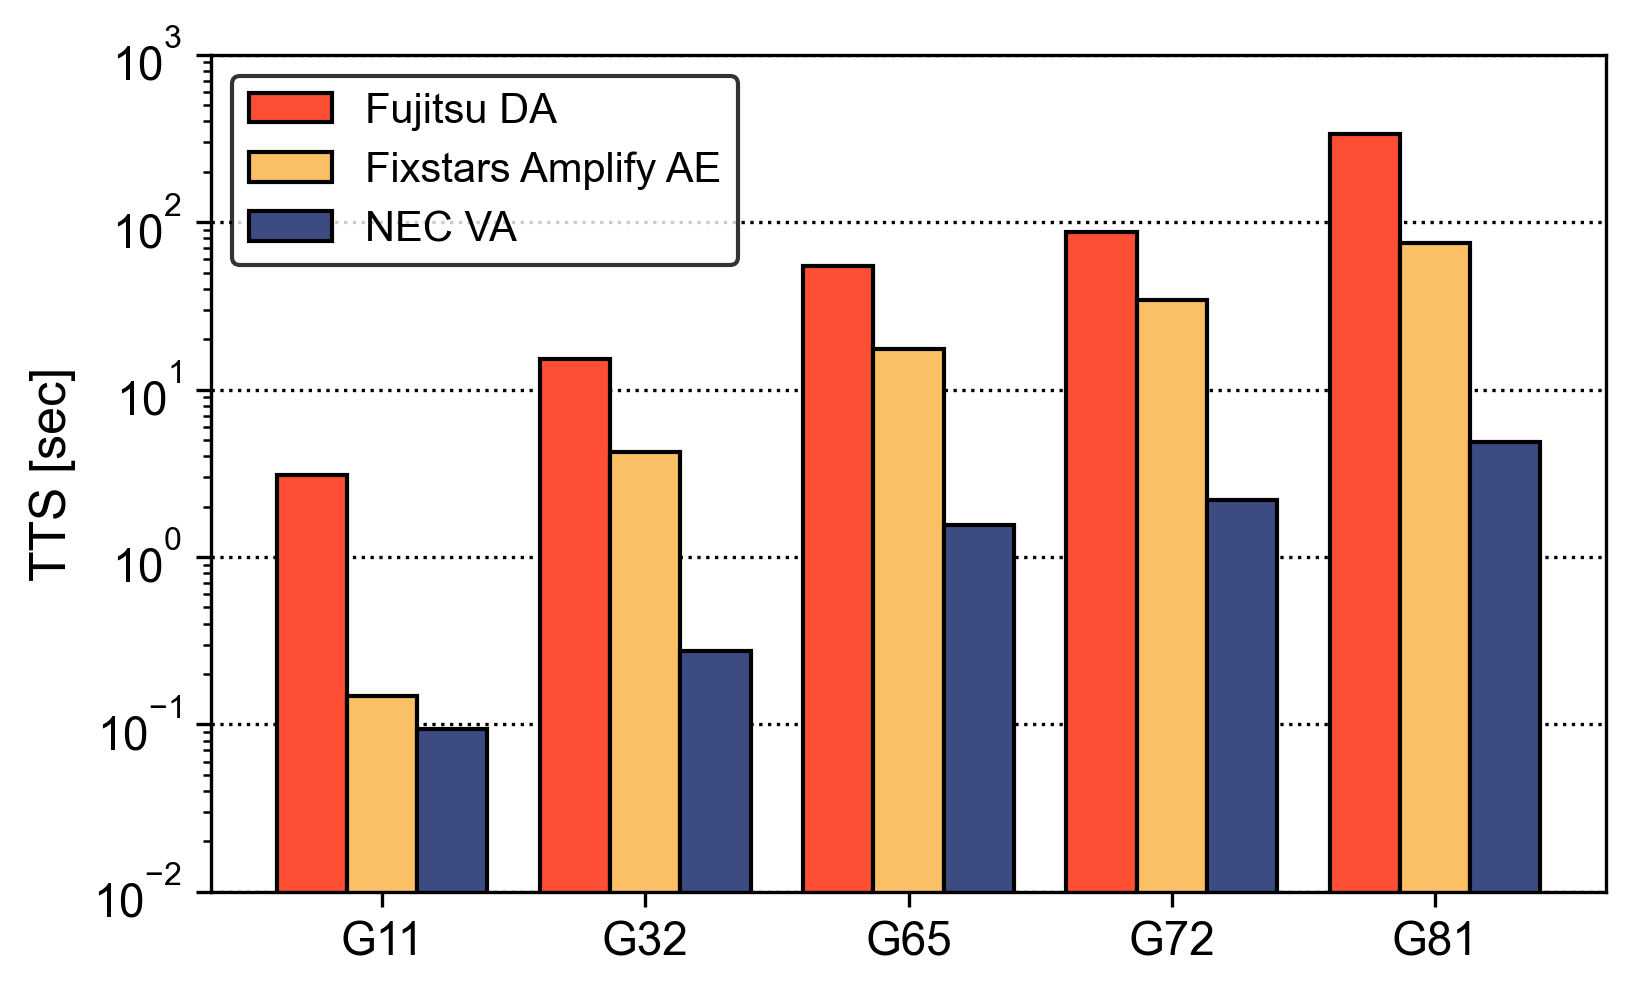
\includegraphics[bb=0 0 700 230, width=15cm]{TTS_Maxcut.png}
\caption{擬似量子アニーリングマシンによるTTSの比較(Maxcut).}
\label{Maxcut_TTS}
\end{figure}

\begin{figure}[ht]
\centering
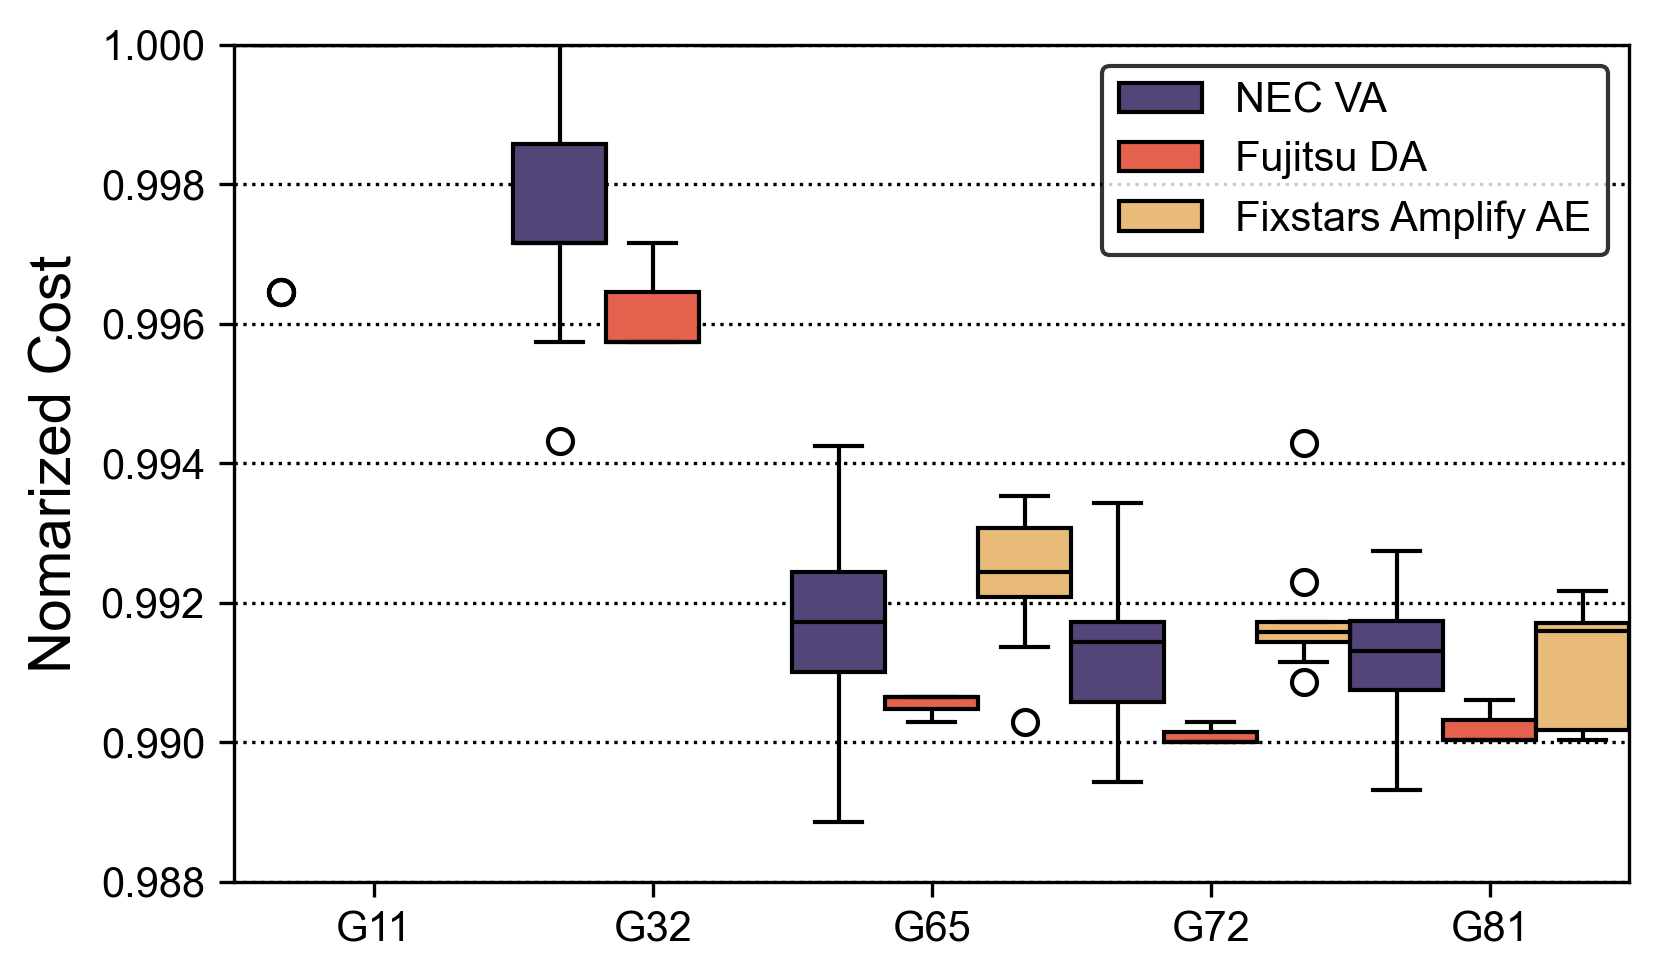
\includegraphics[bb=0 0 700 230, width=15cm]{speed_vs_constraint_Maxcut.png}
\caption{擬似量子アニーリングマシンによる解精度の比較(Maxcut).}
\label{Maxcut_speed_vs_const}
\end{figure}

%4.2.2
\subsubsection{ワンホット制約を持つTSP, QAPによる評価}
\textcolor{blue}{図\ref{TTS_TSP}に, TSPによるTTSの結果を示す. 図\ref{TTS_TSP}に示す通り, Fixstars Amplify AEでは, 200地点以上の問題でTTSが大きく悪化していることが分かる. また図\ref{TSP_speed_vs_const}に, 同実行により得られた解精度分布を示す. 図\ref{TSP_speed_vs_const}より, Fixstars Amplify AEでは200地点以上の問題で解精度が低下し, 目標精度の解に到達しないの解の割合が多くなることが分かる. 従って, 大規模におけるTTSの悪化が正答率の低下に起因していることが分かる. 一方, NEC VA, Fujitsu DAでは, 制約機能を指定したことにより, 大規模においても高い解精度を維持していることが分かる.}

\begin{figure}[ht]
\centering
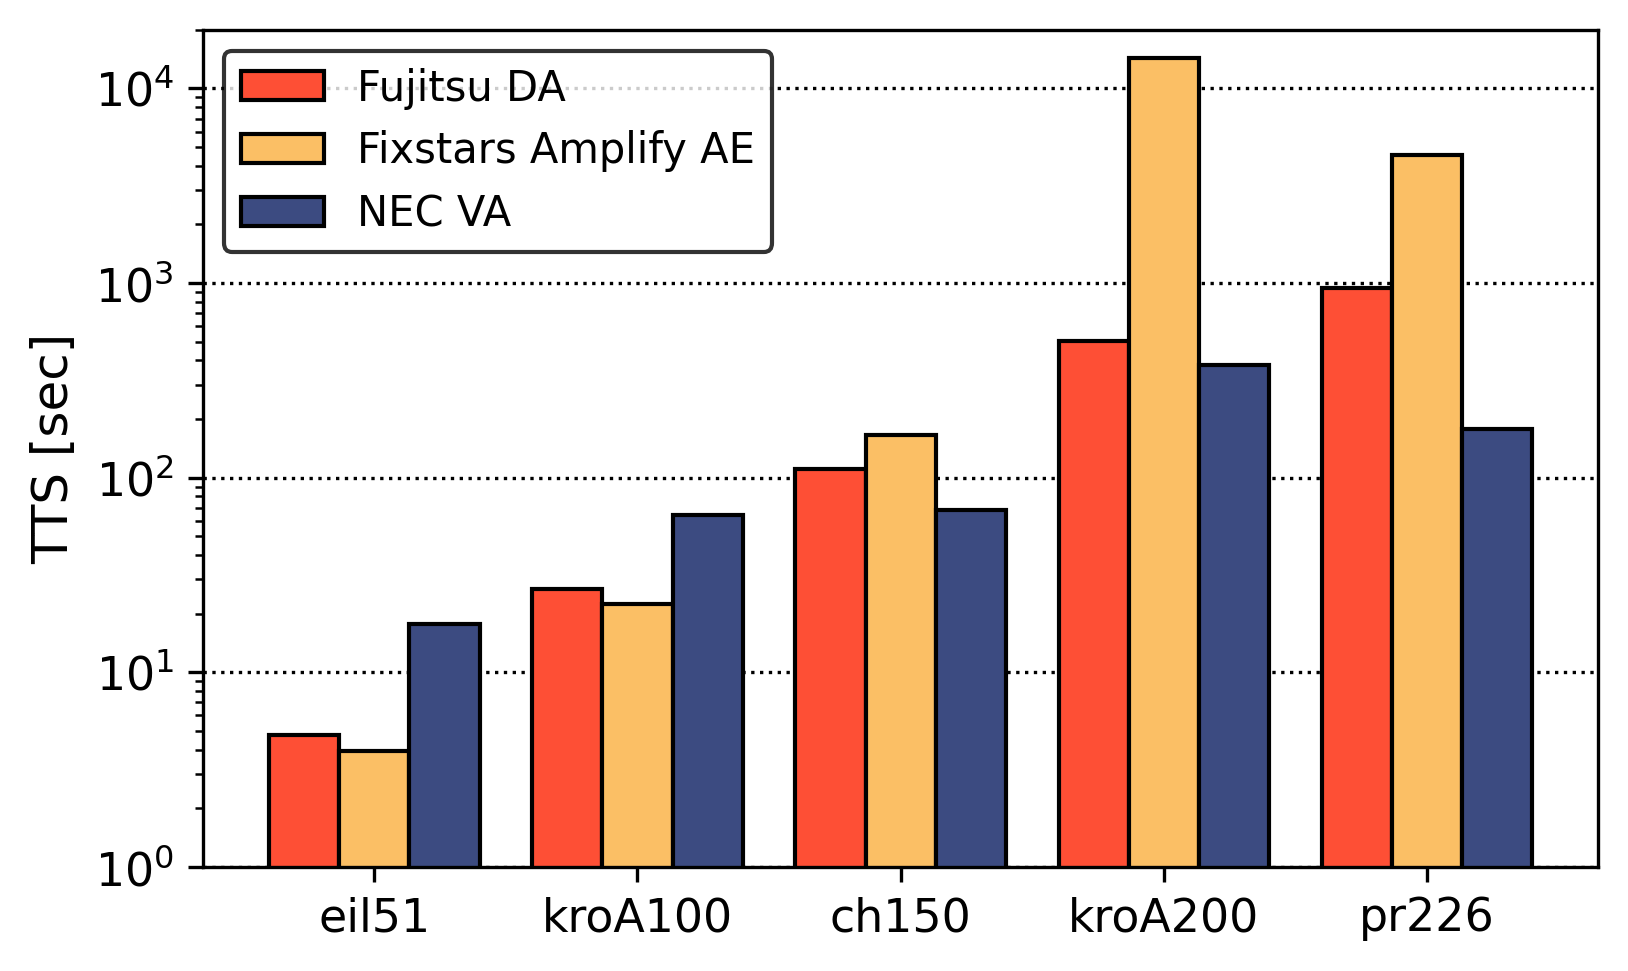
\includegraphics[bb=0 0 700 230, width=15cm]{TTS_TSP.png}
\caption{擬似量子アニーリングマシンによるTTSの比較(TSP).}
\label{TTS_TSP}
\end{figure}

\begin{figure}[ht]
\centering
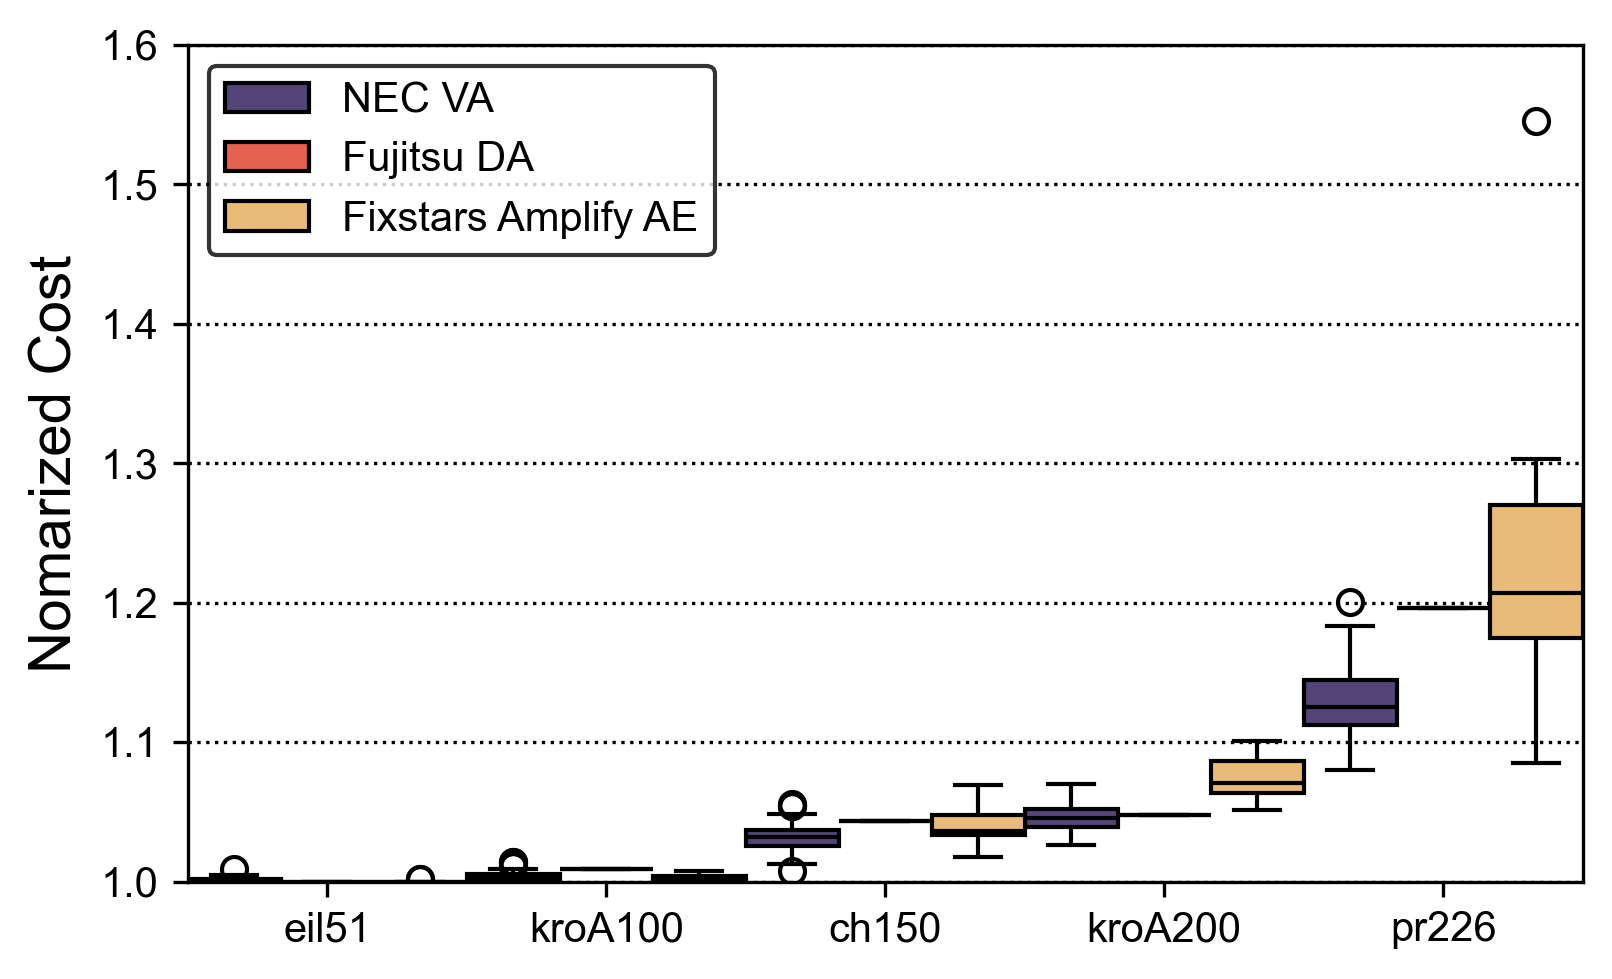
\includegraphics[bb=0 0 700 230, width=15cm]{speed_vs_constraint_TSP.png}
\caption{擬似量子アニーリングマシンによる解精度の比較(TSP).}
\label{TSP_speed_vs_const}
\end{figure}

\textcolor{blue}{図\ref{TTS_QAP}に, QAPによるTTSの結果を示す. 図\ref{TTS_QAP}に示す通り, 全インスタンスにおいて, Fixstars Amplify AEのTTSがNEC VA, Fujitsu DAに対して大きく, グラフが表示されていない150地点の問題では目標精度の解が得られていない. また図\ref{QAP_speed_vs_const}に, 同実行により得られた解精度分布を示す. 図\ref{QAP_speed_vs_const}より, Fixstars Amplify AEでは問題規模の増大に伴い, 目標精度に到達しない解の割合が多くなることが分かる. 一方, NEC VA, Fujitsu DAでは, 制約機能を指定することにより, 大規模においても目標精度を満たす高い精度を維持していることが分かる.}

\begin{figure}[ht]
\centering
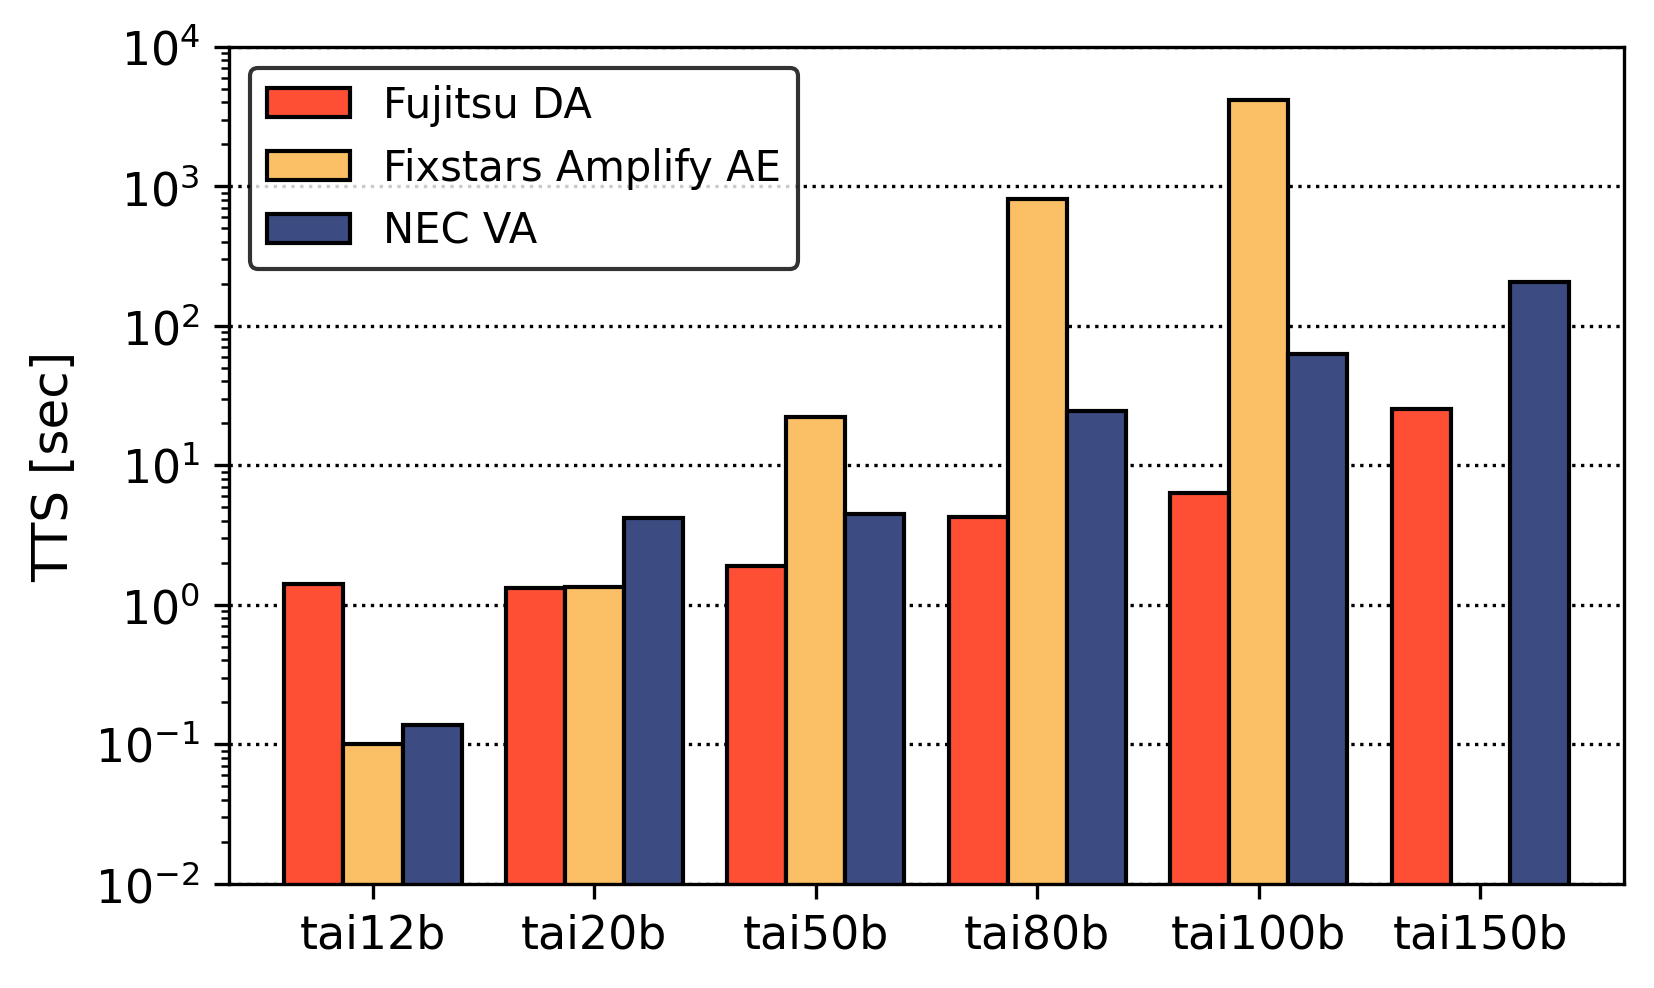
\includegraphics[bb=0 0 700 230, width=15cm]{TTS_QAP.png}
\caption{擬似量子アニーリングマシンによるTTSの比較(QAP).}
\label{TTS_QAP}
\end{figure}

\begin{figure}[ht]
\centering
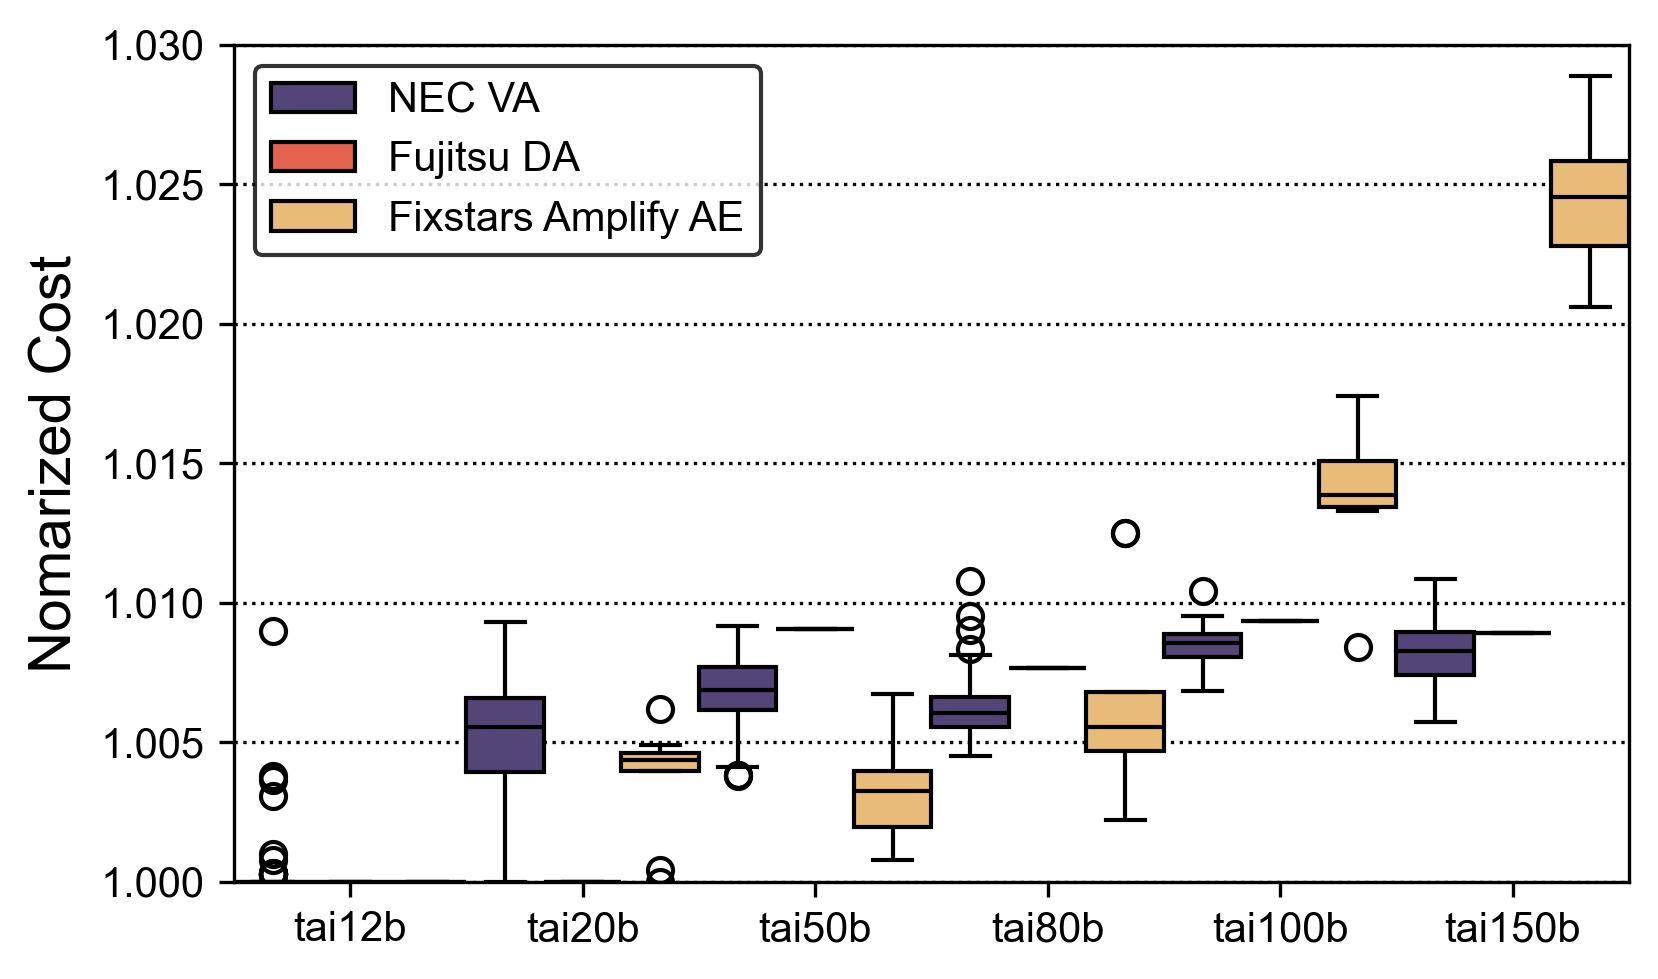
\includegraphics[bb=0 0 700 230, width=15cm]{speed_vs_constraint_QAP.png}
\caption{擬似量子アニーリングマシンによる解精度の比較(QAP).}
\label{QAP_speed_vs_const}
\end{figure}

%4.2.3
\subsubsection{不等式制約を持つQKPによる評価}
\textcolor{blue}{図\ref{TTS_QKP}に, QKPによるTTSの結果を示す. 図\ref{TTS_QKP}に示す通り, jeu\_200\_50\_1, jeu\_300\_50\_1において, NEC VAではTTSが悪化し, Fixstars Amplify AEでは目標精度の解が得られていない. また図\ref{Cost_QKP_All}には, 同実行により得られた解精度分布を示す. 図\ref{Cost_QKP_All}より, Fixstars Amplify AEでは目標精度から大きく低下した領域に解が分布しているのに対して, NEC VA, Fujitsu DAでは全インスタンスで目標精度に到達できることが分かる.}

\begin{figure}[ht]
\centering
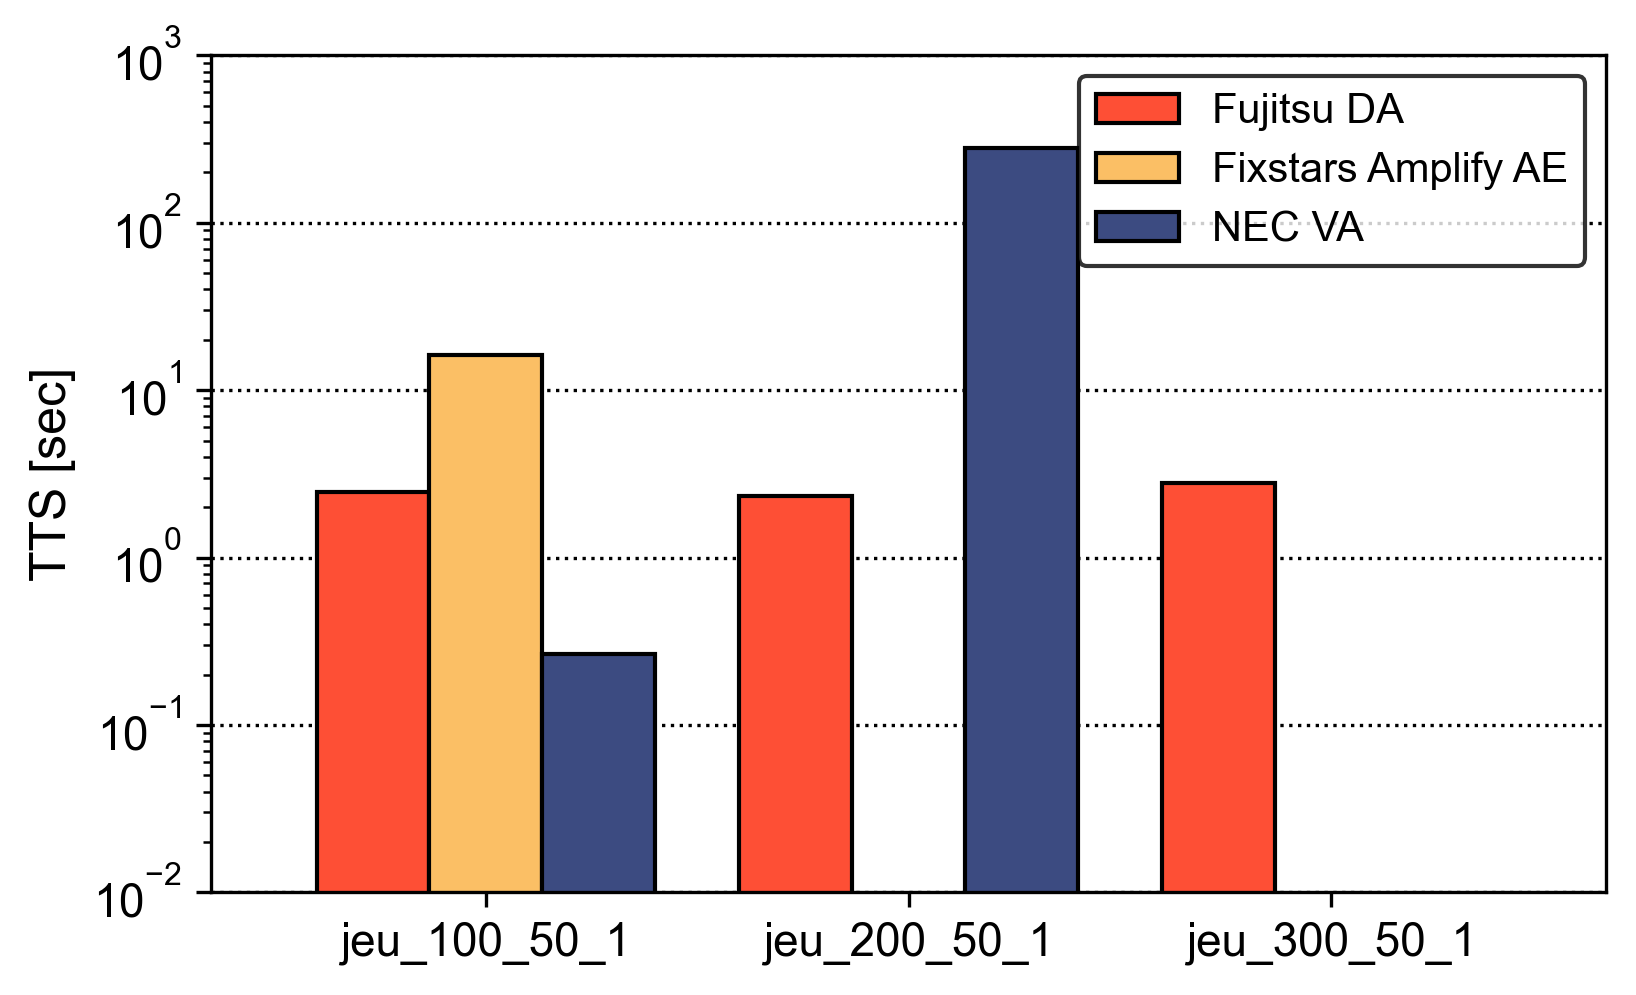
\includegraphics[bb=0 0 700 250, width=15cm]{TTS_QKP.png}
\caption{擬似量子アニーリングマシンによるTTSの比較(QKP).}
\label{TTS_QKP}
\end{figure}

\begin{figure}[ht]
\centering
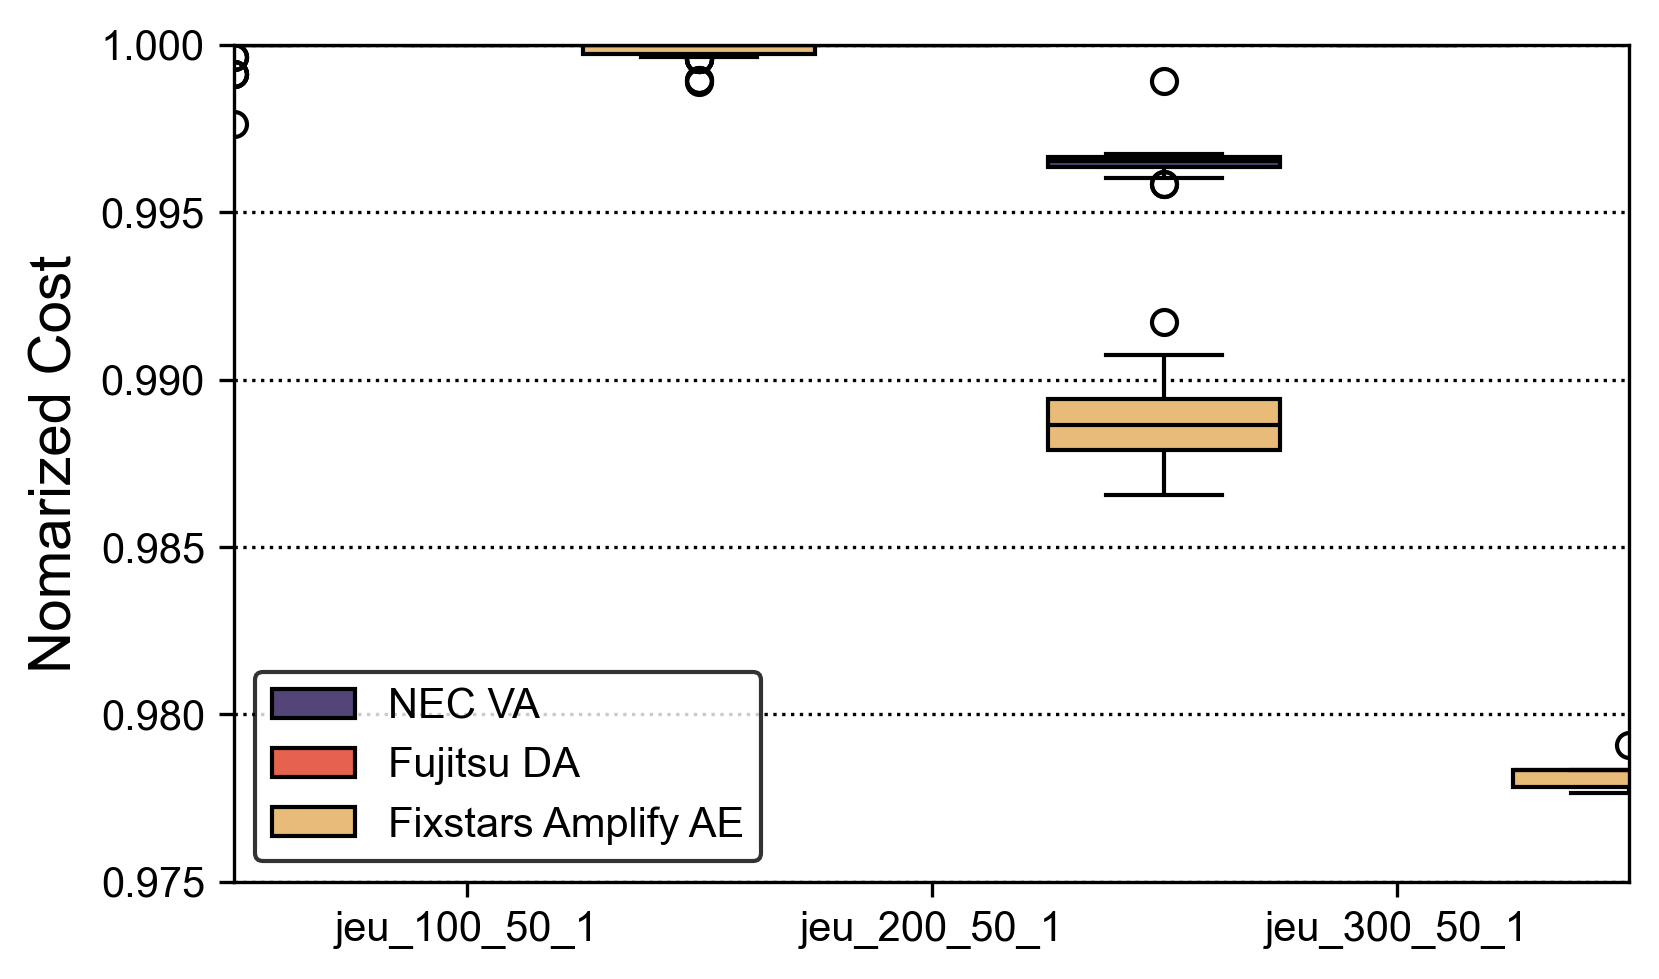
\includegraphics[bb=0 0 700 250, width=15cm]{Cost_QKP_All.png}
\caption{擬似量子アニーリングマシンによる解精度の比較(QKP).}
\label{Cost_QKP_All}
\end{figure}

%4.2.4
\subsubsection{禁止ペア制約を持つMISによる評価}
\textcolor{blue}{図\ref{TTS_MIS}に, MISによるTTSの結果を示す. 図\ref{TTS_MIS}より, 問題規模の増大に応じて, 各擬似量子アニーリングマシンのTTSが増加する傾向にあることが分かる. また図\ref{Cost_MIS_All}には, 同実行により得られた解精度分布を示す. 図\ref{Cost_MIS_All}より, 各擬似量子アニーリングマシンによる全ての実行で最適解に収束していることが分かる. このため, MISでは制約機能を指定せず, ペナルティ関数を含める場合でも高い求解精度を示すことが分かる.}

\begin{figure}[ht]
\centering
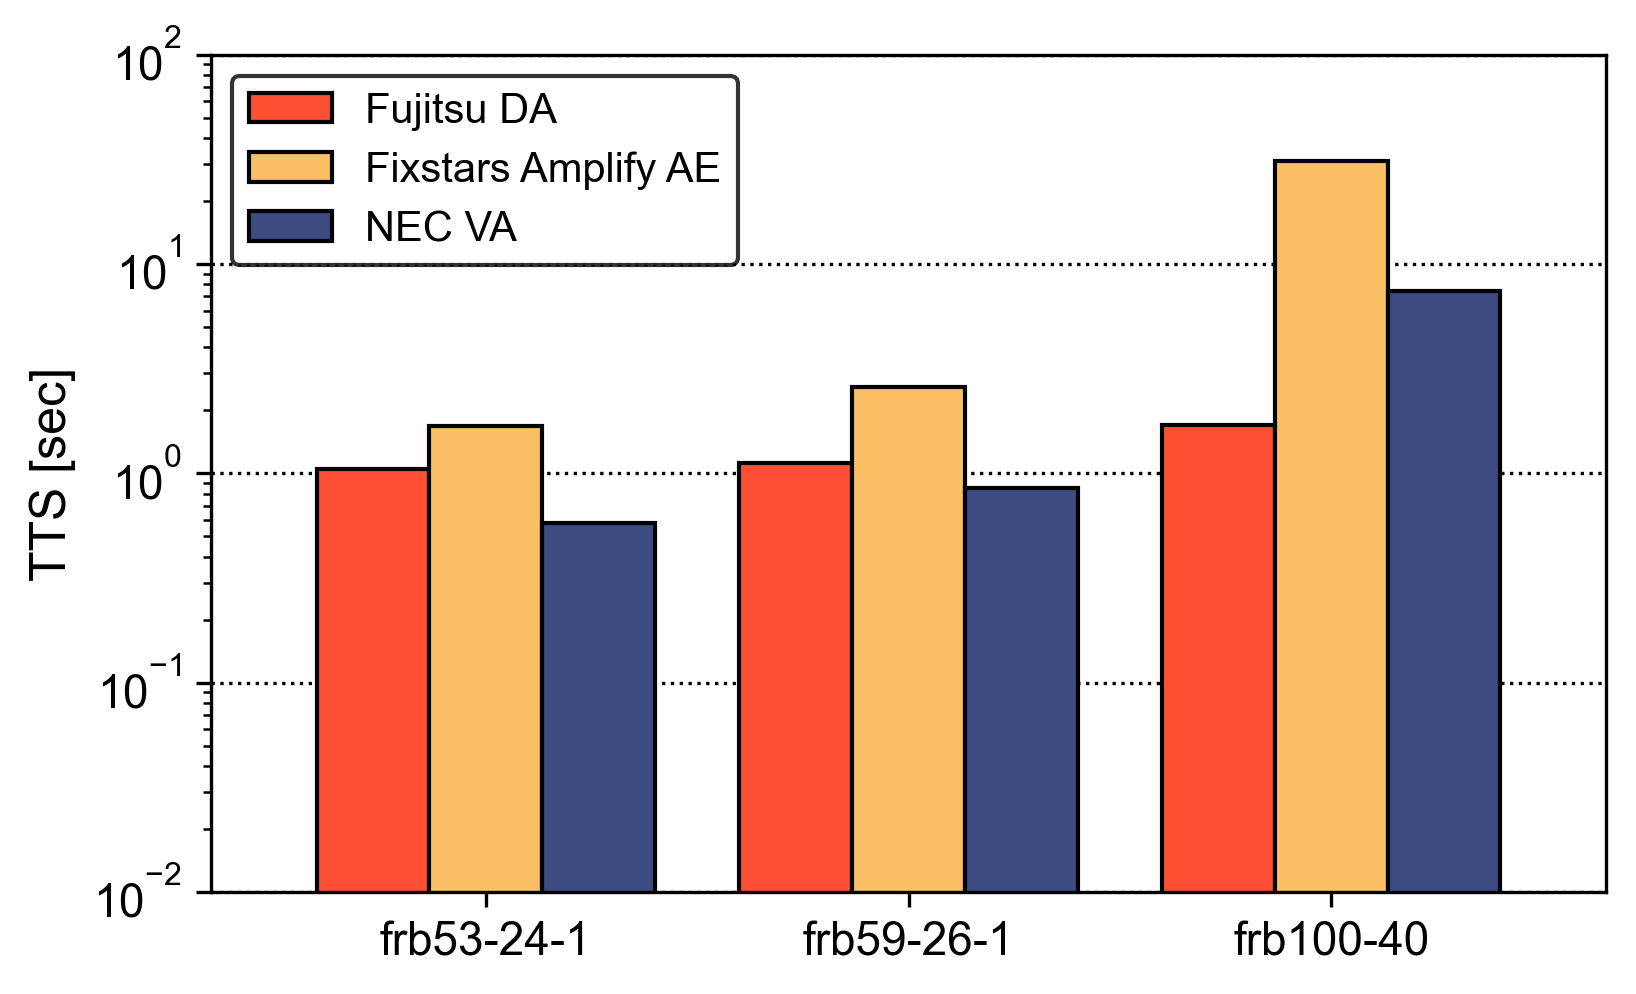
\includegraphics[bb=0 0 700 230, width=15cm]{TTS_MIS.png}
\caption{擬似量子アニーリングマシンによるTTSの比較(MIS).}
\label{TTS_MIS}
\end{figure}

\begin{figure}[ht]
\centering
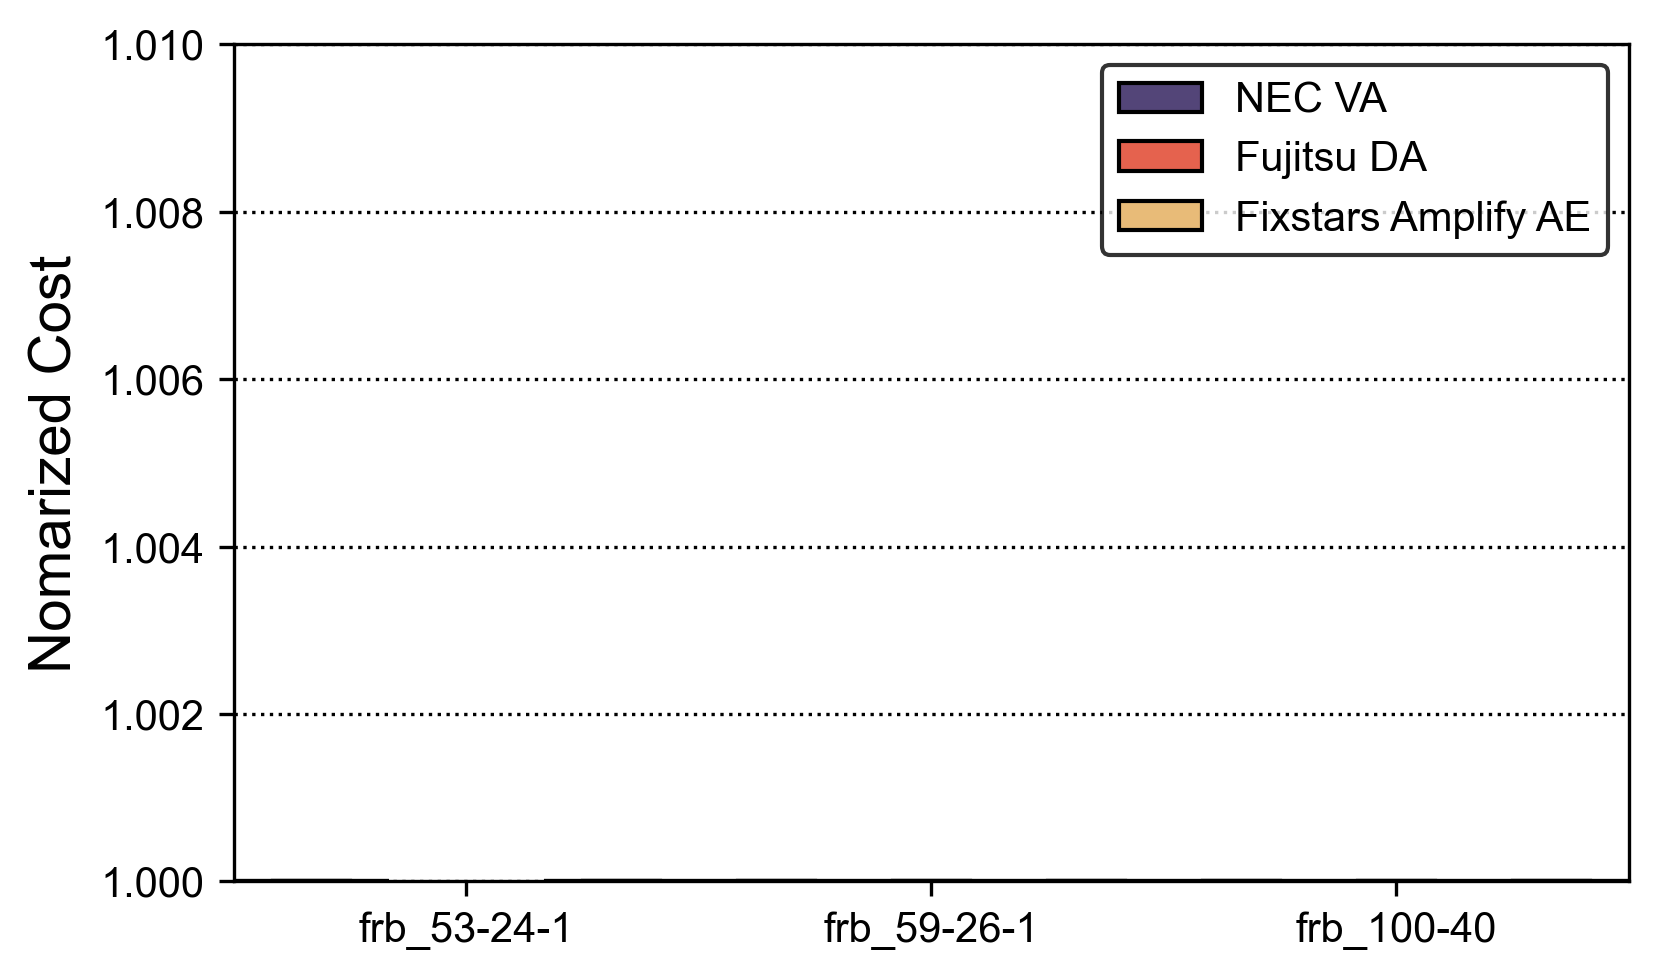
\includegraphics[bb=0 0 700 230, width=15cm]{Cost_MIS_All.png}
\caption{擬似量子アニーリングマシンによる解精度の比較(MIS).}
\label{Cost_MIS_All}
\end{figure}

%6
\section{おわりに}
本稿では, 制約を含まないMaxcut, 及び異なる制約を含むTSP, QAP, QKP, MISを用いて, 擬似量子アニーリングマシンの制約機能の評価を行った. 結果として, ワンホット制約を含むQAP, TSP, 及び不等式制約を含むQKPでは, 擬似量子アニーリングマシンの制約機能を指定した場合に, 制約機能をしない場合と比較して高い解精度を実現できることが分かった. 一方, 禁止ペア制約を含むMISでは, 制約機能の有無によらず, 標準的な擬似量子アニーリングマシンでペナルティ関数を導入した場合でも高い解精度を実現できること分かった. 
% また, 同一の制約条件を含むTSP, QAPに対してNEC VAの異なる制約処理方式を指定した場合, TSPでは制約活用探索, QAPでは制約充足探索がそれぞれ高精度な解に到達できることが分かった. 
これらの結果から, 疑似量子アニーリングマシンの制約機能が, 擬似量子アニーリングマシンのプラットフォームの違い以上に求解性能に大きく寄与しており, 各問題に応じて適切な適切な制約機能を使用することが重要であることが明らかになった.

\begin{acknowledgment}
本研究の一部は,文部科学省「次世代領域研究開発」(高性能汎用計算機高度利用事業費補助金)「量子アニーリングアシスト型次世代スーパーコンピューティング基盤の開発」,文部科学省「次世代計算基盤に係る調査研究」新計算原理調査研究,科研費基盤A\#19H01095,科研費基C\#20K11838,科研費特別研究員奨励費\#22J22908を受けて実施している.
\end{acknowledgment}

\begin{thebibliography}{10}

\bibitem{jobshop}
C. Carugno, Maurizio, F. Dacrema, and Paolo Cremonesi, Evaluating the job shop scheduling problem on a D-wave quantum annealer, {\it Scientific Reports}, {\bf 12}, 6539 (2022).

\bibitem{isc-onoda}
M. Onoda, K. Komatsu, K. Bannai, S. Momose, M. Sato, and H. Kobayashi, Performance Evaluation of Vector Annealing  on Multiple Nodes using  the Traveling Salesperson Problem, {\it International Supercomputing Conference (ISC)} (2025).

\bibitem{portfolio}
W. Sakuler, J. M. Oberreuter, R. Aiolfi, L. Asproni, B. Roman, and J. Schiefer, A real-world test of portfolio optimization with quantum annealing, {\it Quantum Machine Intelligence }, {\bf 7}, 43 (2025).

\bibitem{nishimori}
T. Kadowaki and H. Nishimori, Quantum annealing in the transverse Ising model, {\it Phys. Rev. E}, {\bf 58}, 5355-5363 (1998).

\bibitem{d-wave}
M. W. Johnson, {\it et al}, Quantum annealing with manufactured spins, {\it Nature}, {\bf 473}, 194–198 (2011).

\bibitem{takano}
鷹野芙美代, 鈴木基己, 小林悠記, 荒木拓也. 組合せ最適化問題における制約条件を考慮したQUBOソルバ, {\bf 119}, 314, 15-20 (2019).

\bibitem{Lucas} 
A. Lucas, Ising formulations of many np problems, {\it Frontiers in physics}, {\bf 2}, 5 (2014).

\bibitem{yatabe}
A. Yatabe, Partitioning QUBO with two-way one-hot conditions on traveling salesman problems for city distributions with multiple clusters, {\it Frontiers in Computer Science}, {\bf 6}, 1285244 (2024).

\bibitem{maxcut}
F. Glover and G. Kochenberger, A Tutorial on Formulating QUBO Models Version 1 (2018).

\bibitem{gset}
Gset, https://web.stanford.edu/~yyye/yyye/Gset/.

\bibitem{tsplib}
G. Reinelt, Tsplib|a traveling salesman problem library, {\it FORSA journal on computing}, {\bf 3}, 376 (1991).

\bibitem{qaplib}
R.E. Burkard, S. Karisch and F. Rendl, QAPLIB – A Quadratic Assignment Problem Library, {\it Journal of Global Optimization}, {\bf 10}, 391-403 (1997).

\bibitem{qkplib}
É. Soutif and A. Billionnet, An exact method based on Lagrangian decomposition for the 0–1 quadratic knapsack problems, {\it Eur.J.Oper.Res.}, {\bf 157}, 3, 565–575 (2024).

\bibitem{mislib}
BHOSLIB, https://networkrepository.com/bhoslib.php

\bibitem{va} 
NEC Corporation, 今ある最適化問題解決に - NEC Vector Annealing, https://jpn.nec.com/nec-vector-annealing-service/index.html.

\bibitem{da}
M. Aramon, G. Rosenberg, E. Valiante, T. Miyazawa, H.Tamura,and H.G.Katzgraber, Physics-inspired optimization for quadratic unconstrained problems using a digital annealer, {\it Frontiers in Physics}, {\bf 7}, 48 (2019).

\bibitem{amplify}
Fixstars Corporation, Annealing Machines - The Quantum Computing Cloud - Fixstars Amplify, https://amplify.fixstars.com/en/engine.

\bibitem{kumagai}
M. Kumagai, K. Komatsu, F. Takano, T. Araki, M. Sato, H. Kobayashi, An External Definition of the One-Hot Constraint and Fast QUBO Generation for High-Performance Combinatorial Clustering, {\it International Journal of Networking and Computing}, {\bf 11}, 2 (2021).

\bibitem{komatsu}
K. Komatsu, M. Kumagai, J. Qi, M. Sato, and H. Kobayashi, An externally-constrained ising clustering method for material informatics,  {\it 2021 Ninth International Symposium on Computing and Networking Workshops (CANDARW)}, 201–204 (2021).

\bibitem{kumagai2}
M. Kumagai, K. Komatsu, F. Takano, T. Araki, M. Sato, and H. Kobayashi, Combinatorial clustering based on an externally-defined one-hot constraint, {\it Eighth International Symposium on Computing and Networking (CANDAR)}, 59–68 (2020).

\bibitem{da2}
M. Aramon, G. Rosenberg, E. Valiante, T. Miyazawa, H. Tamura and H. G. Kartzgraber, Physics inspired optimization for quadratic unconstrained problems using a Digital Annealer, {\it Frontiers in Physics}, {\bf 7}, 48 (2019).

\bibitem{da3}
K. Kanda, H. Tamura, M. Begherbeik, P. Ashtari, S. Mousavi and A. Sheikholeslami, イジング最適化を用いた二次割当問題の高速求解, {\it Abstracts. Spring National Conference of Operations Research Society of Japan}, {\bf 2022}, 24-25 (2022).

\bibitem{amplify-da}
P. Codognet, D. Diaz, and S. Abreu, Quantum and Digital Annealing for the Quadratic Assignment Problem, {\it 2022 IEEE International Conference on Quantum Software (QSW)}, 1-8 (2022).

\bibitem{ozeki}
S. Hirama and M. Ohzeki, Efficient Algorithm for Binary Quadratic Problem by Column Generation and Quantum Annealing, {\it Journal of the Physical Society of Japan}, {\bf 92}, 11 (2023).

\bibitem{onoda2}
M. Onoda, K. Komatsu, M. Kumagai, M. Sato, H. Kobayashi, A Constraint Partition Method for Combinatorial Optimization Problems, {\it 2023 IEEE 16th International Symposium on Embedded Multicore/Many-core Systems-on-Chip (MCSoC)} (2023).

\end{thebibliography}

\end{document}
